\documentclass[runningheads]{llncs}

\pagestyle{plain}

%\usepackage[bookmarks]{hyperref}
\usepackage{amsmath,amssymb,xcolor,graphicx,wrapfig,paralist}
\usepackage{algorithmicx,algorithm}
\usepackage[noend]{algpseudocode}
\usepackage{booktabs}
\usepackage{proof}
\usepackage{tikz}
\usepackage{csquotes}
\usepackage{graphics}
\usepackage{stmaryrd}
\usepackage{soul}
\usepackage{array}
%\usepackage{titlesec}
\usepackage{sectsty}
% \usepackage{amsmath,amsthm}

\usepackage{ellipsis, mparhack, ragged2e} % bugfixing
\usepackage[l2tabu, orthodox]{nag} % avoid typical LaTeX errors

\usepackage{tabu,multirow}
\usepackage{xparse}
\usepackage{mathtools}
\usepackage{environ}
\usepackage{lscape}

\usepackage{url}

\usepackage[english]{babel}
% \usepackage[latin1]{inputenc}
% \usepackage[pdftex]{hyperref}

%\usepackage[caption=false]{subfig}
%\usepackage{caption}
\usepackage{subcaption}
\captionsetup{compatibility=false}

\usepackage{algorithm}
\usepackage{algpseudocode}

\usepackage{marginfix}
\usepackage{xifthen}

\usepackage[protrusion=true,expansion=true]{microtype}

\usepackage{listings}
\lstdefinestyle{customJ}{
  belowcaptionskip=1\baselineskip,
  breaklines=true,
  frame=L,
  xleftmargin=\parindent,
  language=Java,
  showstringspaces=false,
  basicstyle=\footnotesize\ttfamily,
  keywordstyle=\bfseries\color{green!40!black},
  commentstyle=\itshape\color{purple!40!black},
  identifierstyle=\color{blue},
  stringstyle=\color{orange},
}

\usepackage{afterpage}
\newcommand\blankpage{%
    \null
    \thispagestyle{empty}%
    \newpage}

\renewcommand{\arraystretch}{1.2}

\usepackage{xfrac}

\usepackage{multirow}

%\newcommand{\gls}[1]{#1}
\usetikzlibrary{shapes,positioning,arrows,calc,automata,matrix,fit}
\tikzstyle{state}+=[minimum size = 6mm, inner sep=0,outer sep=1]
\tikzset{->,>=stealth'}
% == TODOs
\newcommand{\todojan}[1]{\todo{\color{blue}\textbf{Jan:\\}#1}}
\newcommand{\todojulia}[1]{\todo{\highlight{Ju:\\}#1}}
\newcommand{\todopranav}[1]{\todo{\textbf{Pranav:\\}#1}}
\newcommand{\todomaxi}[1]{\todo{\textbf{Maxi:\\}#1}}

\newcommand{\todoin}[1]{{\color{red}#1}}

% == HIGHLIGHTING

% highlight for text mode
\newcommand{\highlighttext}[1]{\colorbox{black!15}{#1}}

% highlight for math mode
\newcommand{\highlight}[1]{\colorbox{black!15}{$\displaystyle#1$}}

% == ALGORITHMS
\renewcommand{\algorithmicrequire}{\textbf{Input:}}
\renewcommand{\algorithmicensure}{\textbf{Output:}}
%\algrenewcommand{\algorithmiccomment}[1]{\hskip1.5em \textbackslash *  #1 * \textbackslash}
%\renewcommand{\algorithmiccomment}[1]{\bgroup\hfill\tiny//~#1\egroup}

%define a marking command
\newcommand*{\tikzmk}[1]{\tikz[remember picture,overlay,] \node (#1) {};\ignorespaces}
%define a boxing command, argument = colour of box
\newcommand{\boxit}[1]{\tikz[remember picture,overlay]{\node[yshift=3pt,fill=#1,opacity=.25,fit={(A)($(B)+(.95\linewidth,.8\baselineskip)$)}] {};}\ignorespaces}
%define some colours according to algorithm parts (or any other method you like)
\colorlet{pink}{red!40}
\colorlet{blue}{cyan!60}

% == TABLES
\newcolumntype{L}{X}
\newcolumntype{R}{>{\raggedleft\arraybackslash}X}
\newcolumntype{C}{>{\centering\arraybackslash}X}

% Hidden column
\newcolumntype{H}{>{\setbox0=\hbox\bgroup}c<{\egroup}@{}}

% == GRAPHICS
\DeclareGraphicsExtensions{.pdf, .png, .jpg}

% == LATEX
\newcommand\numberthis{\addtocounter{equation}{1}\tag{\theequation}}

% == THEOREMS
%\newtheorem{theo}{Theorem}[section]
\newtheorem{cor}{Corollary}%[lemma]
\newtheorem{ass}{Assumption}%[lemma]
%\newtheorem{lem}[theo]{Lemma}
  
\def\qedtriangle{\hspace{\stretch1}\ensuremath\triangleleft}
\def\qedsquare{\hspace{\stretch1}\ensuremath\square}

% == SPACE

%\usepackage{microtype}
%\renewcommand{\baselinestretch}{0.975} % >=0.97

%\newcommand{\spacefu}{\vspace*{-1.2em}}
%\newcommand{\spacefl}{\vspace*{-0.8em}}
\newcommand{\myspace}{\vspace*{-0.5em}}

% == TODO

\NewDocumentCommand{\todo}{m}{%
	% Add to todo list
	\begin{tikzpicture}[remember picture, baseline=-0.75ex]%
	\node [coordinate] (inText) {};%
	\end{tikzpicture}%
	%
	% Make the margin par
	\marginpar{%
		\begin{tikzpicture}[remember picture, font=\scriptsize]%
		\draw node[draw=red, text width = 3.5cm, inner sep=0.3mm] (inNote){#1};%
		\end{tikzpicture}%
	}%
	\begin{tikzpicture}[remember picture, overlay]%
	\draw[draw=red]%
	([yshift=-0.2cm] inText)%
	% -| ([xshift=-0.05cm] inNote.west)%
	-| (inNote.south);%
	\end{tikzpicture}%
}%
% == SYMBOLS

\RequirePackage{marvosym}
\providecommand{\contradiction}{\Lightning}


% == BOOLEAN

\newcommand{\boolor}{\vee}
\newcommand{\booland}{\wedge}
\newcommand{\boolOr}{\bigvee}
\newcommand{\boolAnd}{\bigwedge}
\newcommand{\boolnot}{\lnot}


% == BASIC OPERATORS

\DeclarePairedDelimiter{\delimabs}{\lvert}{\rvert}
\DeclarePairedDelimiter{\delimnorm}{\lVert}{\rVert}
\DeclarePairedDelimiter{\delimpospart}{\lgroup}{\rgroup^+}
\DeclarePairedDelimiter{\delimnegpart}{\lgroup}{\rgroup^-}
\DeclarePairedDelimiterX{\deliminner}[2]{\lange}{\rangle}{#1, #2}
\DeclarePairedDelimiter{\delimcardinality}{\lvert}{\rvert}
\DeclarePairedDelimiter{\delimset}{\lbrace}{\rbrace}
\DeclarePairedDelimiter{\delimtuple}{(}{)}
\DeclarePairedDelimiter{\delimlistt}{[}{]}
\DeclarePairedDelimiter{\delimfun}{(}{)}

\NewDocumentCommand{\abs}{sm}{\IfBooleanTF{#1}{\delimabs{#2}}{\delimabs*{#2}}}
\NewDocumentCommand{\norm}{sm}{\IfBooleanTF{#1}{\delimnorm{#2}}{\delimnorm*{#2}}}
\NewDocumentCommand{\pospart}{sm}{\IfBooleanTF{#1}{\delimpospart{#2}}{\delimpospart*{#2}}}
\NewDocumentCommand{\negpart}{sm}{\IfBooleanTF{#1}{\delimnetpart{#2}}{\delimnetpart*{#2}}}
\NewDocumentCommand{\inner}{sm}{\IfBooleanTF{#1}{\deliminner{#2}}{\deliminner*{#2}}}
\NewDocumentCommand{\cardinality}{sm}{\IfBooleanTF{#1}{\delimcardinality{#2}}{\delimcardinality*{#2}}}
\NewDocumentCommand{\set}{sm}{\IfBooleanTF{#1}{\delimset*{#2}}{\delimset{#2}}}
\NewDocumentCommand{\tuple}{sm}{\IfBooleanTF{#1}{\delimtuple{#2}}{\delimtuple*{#2}}}
\NewDocumentCommand{\closure}{sm}{\IfBooleanTF{#1}{\delimclosure{#2}}{\delimclosure*{#2}}}
\NewDocumentCommand{\listt}{sm}{\IfBooleanTF{#1}{\delimlistt{#2}}{\delimlistt*{#2}}}
\NewDocumentCommand{\fun}{smm}{\IfBooleanTF{#1}{{#2}\delimfun{#3}}{{#2}\delimfun*{#3}}}
\NewDocumentCommand{\funMacro}{smm}{\IfNoValueTF{#3}{#1}{\fun{#2}{#3}}}

\DeclareMathOperator{\ExistsOp}{\exists}
\DeclareMathOperator{\ForallOp}{\forall}

\NewDocumentCommand{\Exists}{gg}{\IfNoValueTF{#1}{\ExistsOp}{\ExistsOp #1. \, #2}}
\NewDocumentCommand{\Forall}{gg}{\IfNoValueTF{#1}{\ForallOp}{\ForallOp #1. \, #2}}

\DeclarePairedDelimiter\ceil{\lceil}{\rceil}
\DeclarePairedDelimiter\floor{\lfloor}{\rfloor}


% == SETS OPERATORS

\newcommand{\setcomplement}[1]{{#1}^c}
\newcommand{\powerset}[1]{\mathcal{P}(#1)}

\newcommand{\unionSym}{\cup}
\newcommand{\unionBin}{\mathbin{\unionSym}}
\newcommand{\strictunionSym}{\dot{\unionSym}}
\newcommand{\strictunionBin}{\mathbin{\dot{\unionSym}}}
\newcommand{\intersectionSym}{\cap}
\newcommand{\intersectionBin}{\mathbin{\intersectionSym}}
\newcommand{\UnionSym}{\bigcup}
\newcommand{\UnionBin}{\mathbin{\UnionSym}}
\newcommand{\strictUnionSym}{\dot{\UnionSym}}
\newcommand{\strictUnionBin}{\mathbin{\strictUnionSym}}
\newcommand{\IntersectionSym}{\bigcap}
\newcommand{\IntersectionBin}{\mathbin{\IntersectionSym}}

\newcommand{\union}{\unionBin}
\newcommand{\strictunion}{\strictunionBin}
\newcommand{\intersection}{\intersectionBin}
\newcommand{\Union}{\UnionSym}
\newcommand{\strictUnion}{\strictUnionSym}
\newcommand{\Intersection}{\IntersectionSym}


% == BASIC SETS

\newcommand{\Continuous}{C}
\newcommand{\Sobolev}{\mathcal{W}}
\newcommand{\Naturals}{\mathbb{N}}
\newcommand{\Domain}{\mathfrak{D}}
\newcommand{\Measures}{\mathcal{M}}
\newcommand{\Lebesgue}{\mathcal{L}}
\newcommand{\Hilb}{H}
\newcommand{\Reals}{\mathbb{R}}
\newcommand{\Orlicz}{{\tilde{\Lebesgue}}}
\newcommand{\Distributions}{\mathcal{D}}


% == LIMITS

\NewDocumentCommand{\convto}{G{}}{\xrightarrow{#1}}
\NewDocumentCommand{\weakto}{G{}}{\xrightharpoonup{#1}}
\NewDocumentCommand{\weakstarto}{G{}}{\xrightharpoonup[*]{#1}}

% == OPERATORS

\newcommand{\gradient}{\nabla}
\newcommand{\laplacian}{\Delta}
 \DeclareDocumentCommand{\diff}{D<>{} O{}  D(){}}{\Delta_{#1}^{#2}\ifthenelse{\isempty{#3}}{}{(#3)}}
\newcommand{\boundary}{\partial}
\DeclareMathOperator{\divergence}{div}
\DeclareMathOperator{\distance}{dist}
\DeclareMathOperator{\esssup}{ess sup}
\DeclareMathOperator{\supp}{supp}
\DeclareMathOperator{\capacity}{cap}
\DeclareMathOperator{\signum}{signum}
\DeclareMathOperator{\id}{id}
\DeclareMathOperator{\const}{const}
\DeclareMathOperator{\loc}{loc}
\DeclareMathOperator*{\argmax}{arg\, max}
\DeclareMathOperator*{\argmin}{arg\, min}
\DeclareDocumentCommand{\post}{D<>{} O{} D(){}}{\mathsf{Post}_{#1}^{#2}\ifthenelse{\isempty{#3}}{}{(#3)}}
\DeclareMathOperator{\leaves}{\mathbin{\mathop{exits}}}
\newcommand{\leaving}{exiting}
\DeclareMathOperator{\stays}{\mathbin{\mathop{\mathsf{stays\_in}}}}
\newcommand{\eqdef}{\vcentcolon=}
\newcommand{\defeq}{=\vcentcolon}

\newcommand{\qee}{\hfill$\triangle$} % quod erat exemplandum % TODO del

% == LOGIC

\newcommand{\ltl}{\operatorname{LTL}}
\newcommand{\ctl}{\operatorname{CTL}}
\newcommand{\pctl}{\operatorname{pCTL}}
\newcommand{\Next}{\varbigcirc}
\newcommand{\until}{\, \mathcal{U}}
\newcommand{\wrel}{\mathcal{W}}
\newcommand{\lang}[1]{\mathcal{L}(#1)}
\newcommand{\reach}{\Diamond}
\newcommand{\alws}{\Box}
\newcommand{\true}{\mathsf{true}}
\newcommand{\false}{\mathsf{false}}
\newcommand{\turn}{\mathsf{turn}}
\newcommand{\PQ}{\mathrm{PQ}}

% == COMPLEXITY
\newcommand{\NP}{\mathbf{NP}}
\newcommand{\NEXP}{\mathbf{NEXP}}
\newcommand{\PSPACE}{\mathbf{PSPACE}}

% == PROBABILITY
\NewDocumentCommand{\distributions}{d()}{\funMacro{\mathcal{D}}{#1}}
\newcommand{\dirac}[1]{\delta_{#1}}
\newcommand{\probability}{\mathbb{P}}
\newcommand{\expectation}{\mathbb{E}}

% == MC, MPD, Games

\newcommand{\gain}{g} %value
\newcommand{\bias}{b}
\newcommand{\stat}{q}
\newcommand{\outcomes}{\mathcal{O}}
\newcommand{\salgebra}{\mathcal{F}}
\newcommand{\mevent}{\mathcal{E}}
\newcommand{\pmin}{p_{\min}}
\newcommand{\rmax}{r_{\max}}
\newcommand{\MECs}{\mathsf{MEC}}
\newcommand{\GCs}{\mathsf{GC}}
\DeclareDocumentCommand{\val}{D<>{} O{}  D(){} t'}{\mathsf{V}_{#1}^{\IfBooleanTF{#4}{\prime #2}{#2}}\ifthenelse{\isempty{#3}}{}{(#3)}}
\DeclareDocumentCommand{\ub}{D<>{} O{}  D(){} t'}{\mathsf{U}_{#1}^{\IfBooleanTF{#4}{\prime #2}{#2}}\ifthenelse{\isempty{#3}}{}{(#3)}}
\DeclareDocumentCommand{\gub}{D<>{} O{}  D(){} t'}{\mathsf{G}_{#1}^{\IfBooleanTF{#4}{\prime #2}{#2}}\ifthenelse{\isempty{#3}}{}{(#3)}}
\DeclareDocumentCommand{\lb}{D<>{} O{}  D(){} t'}{\mathsf{L}_{#1}^{\IfBooleanTF{#4}{\prime #2}{#2}}\ifthenelse{\isempty{#3}}{}{(#3)}}
\DeclareDocumentCommand{\game}{D<>{} O{} D(){} t'}{\mathsf{G}_{#1}^{\IfBooleanTF{#4}{\prime}{}#2}\ifthenelse{\isempty{#3}}{}{(#3)}}
\DeclareDocumentCommand{\transition}{D<>{} O{} D(){}}{\rightarrow_{#1}^{#2}\ifthenelse{\isempty{#3}}{}{(#3)}}


\newcommand{\Ts}{\mathcal{T}}
\newcommand{\MC}{\mathsf{M}}
\newcommand{\Mdp}{\mathcal{M}}
\newcommand{\Pm}{\mathbf{P}}
\newcommand{\SG}{\textrm{SG}}
\newcommand{\SGs}{\textrm{SGs}}
\newcommand{\M}{\mathsf{M}}
\DeclareDocumentCommand{\G}{D<>{} O{} t' D(){}}{\mathsf{G}_{#1}^{\IfBooleanTF{#3}{\prime}{}#2}\ifthenelse{\isempty{#4}}{}{(#4)}}
\DeclareDocumentCommand{\exGame}{D<>{} O{} t'  D(){}}{\mathsf{G}_{#1}^{\IfBooleanTF{#3}{\prime}{}#2}\ifthenelse{\isempty{#4}}{}{(#4)}=(\states<#1>[\IfBooleanTF{#3}{\prime}{}#2],\states<\Box\ifthenelse{\isempty{#1}}{}{,#1}>[\IfBooleanTF{#3}{\prime}{}#2],\states<\circ\ifthenelse{\isempty{#1}}{}{,#1}>[\IfBooleanTF{#3}{\prime}{}#2],\istate<#1>[\IfBooleanTF{#3}{\prime}{}#2],\actions<#1>[\IfBooleanTF{#3}{\prime}{}#2],\Av<#1>[\IfBooleanTF{#3}{\prime}{}#2],\trans<#1>[\IfBooleanTF{#3}{\prime}{}#2])}


\newcommand{\ap}{Ap}
\DeclareDocumentCommand{\states}{D<>{} O{}  t'}{\mathsf{S}_{#1}^{\IfBooleanTF{#3}{\prime~#2}{#2}}}
\DeclareDocumentCommand{\state}{D<>{} O{}  t'}{\mathsf{s}_{#1}^{\IfBooleanTF{#3}{\prime #2}{#2}}}
\DeclareDocumentCommand{\istate}{D<>{} O{} t'}{\mathsf{s}_{0\ifthenelse{\isempty{#1}}{}{,#1}}^{\IfBooleanTF{#3}{\prime~#2}{#2}}}
\newcommand{\inv}{\nu}
\newcommand{\lab}{L}

\newcommand{\edges}{E}
\newcommand{\statesone}{S^N}
\newcommand{\statestwo}{S_2}
\newcommand{\statesp}{S^P}
\newcommand{\initstate}{\state<0>}
\newcommand{\initdist}{\mu}
\DeclareDocumentCommand{\trans}{D<>{} O{} t' D(){} D(){}}{\delta{#1}^{\IfBooleanTF{#3}{\prime}{}#2}\ifthenelse{\isempty{#4}}{}{(#4)}\ifthenelse{\isempty{#5}}{}{(#5)}}
\DeclareDocumentCommand{\Av}{D<>{} O{} t' D(){}}{\mathsf{Av}_{#1}^{\IfBooleanTF{#3}{\prime}{}#2}\ifthenelse{\isempty{#4}}{}{(#4)}}
\newcommand{\rew}{r}
\DeclareDocumentCommand{\F}{D<>{} O{} t' D(){}}{\mathsf{F}_{#1}^{\IfBooleanTF{#3}{\prime}{}#2}\ifthenelse{\isempty{#4}}{}{(#4)}}
\newcommand{\lu}{\hat{l},\hat{u}}

% = paths and strategies
\newcommand{\Path}{\rho}
\DeclareDocumentCommand{\Path}{D<>{} O{} t' D(){}}{\path<#1>[#2]\IfBooleanTF{#3}{'}{}(#4)}
\DeclareDocumentCommand{\path}{D<>{} O{} t' D(){}}{\rho_{#1}^{\IfBooleanTF{#3}{\prime}{}#2}\ifthenelse{\isempty{#4}}{}{(#4)}}
\newcommand{\fpath}{\mathsf{w}}
\DeclareDocumentCommand{\Paths}{D<>{} O{} t' D(){}}{\Omega_{#1}^{\IfBooleanTF{#3}{\prime}{}#2}\ifthenelse{\isempty{#4}}{}{(#4)}}
\newcommand{\straa}{\sigma}
\newcommand{\straas}{\Sigma}
\newcommand{\strab}{\tau}
\newcommand{\strabs}{\Tau}
\newcommand{\plays}{\mathsf{Plays}}
\newcommand{\play}{\mathsf{Play}}
\newcommand{\last}[1]{\text{last}(#1)}%{#1\mathord\downarrow}
\DeclareDocumentCommand{\strategy}{D<>{} O{} D(){}
  t*}{{\IfBooleanTF{#4}{\tau}{\sigma}}_{#1}^{#2}\ifthenelse{\isempty{#3}}{}{(#3)}}

% = probability

\newcommand{\inits}{\hat s}
\DeclareDocumentCommand{\actions}{D<>{} O{} t' d()}{{\IfNoValueTF{#4}{\mathsf{A}}{\fun{\mathsf{A}}{#4}}}_{#1}^{\IfBooleanTF{#3}{\prime~#2}{#2}}}
\DeclareDocumentCommand{\action}{D<>{} O{} t'}{\mathsf{a}_{#1}^{\IfBooleanTF{#3}{\prime#2}{#2}}}
\newcommand{\pat}{\omega}
\newcommand{\Pat}{\mathsf{Runs}}
\newcommand{\fpat}{w}
\newcommand{\mem}{\mathsf{M}}
\newcommand{\Cone}{\mathsf{Cone}}
\newcommand{\calF}{\mathcal{F}}
\newcommand{\mec}{\mathsf{MEC}}
\newcommand{\scc}{\mathsf{SCC}}
\newcommand{\ec} {\mathsf{EC}}
\newcommand{\bscc}{\mathsf{BSCC}}

\newcommand{\attractor}{\mathsf{prob1}}
\newcommand{\pr}{\mathbb P}
\renewcommand{\Pr}[3]{\pr^{#1}\hspace{-0.16em}\left[{#3}\right]}   %\Pr{strat}{state}{event}
\newcommand{\PrS}[3]{\pr^{#1}_{#2}\hspace{-0.16em}\left[{#3}\right]}   %\Pr{strat}{state}{event}
\newcommand{\expected}{\mathbb{E}}
\newcommand{\expsucc}{\expected_\trans}
\newcommand{\Ex}[3]{\expected^{#1}_{#2}\hspace{-0.16em}\left[{#3}\right]}   %\Ex{strat}{state}{f}
\newcommand{\ExS}[3]{\expected^{#1}_{#2}\hspace{-0.16em}\left[{#3}\right]}   %\Ex{strat}{state}{f}


% == LOCAL

\newcommand{\push}{\mathrm{push}}
\newcommand{\pop}{\mathrm{pop}}
\newcommand{\topx}{\mathrm{top}}


\newcommand{\reward}{\vec{r}}
\newcommand{\ex}{\vecl{exp}}
\newcommand{\sat}{\vecl{sat}}
\newcommand{\satscalar}{\mathit{sat}}
\newcommand{\psat}{\vecl{pr}}%{\vec{p^{sat}}}
\newcommand{\psatscalar}{\mathit{pr}}%{\mathit{p^{sat}}}

\newcommand{\lrLim}[1]{\mathrm{lr}(#1)}  %\lr{rew}{run}
\newcommand{\lrSf}[1]{\mathrm{lr}_{\mathrm{sup}}(#1)}  %\lrS{rew}{run}
\newcommand{\lrIf}[1]{\mathrm{lr}_{\mathrm{inf}}(#1)}  %\lrI{rew}{run}
\newcommand{\lrInf}{\mathrm{lr}^{\mathrm{inf}}}  %\lrI{rew}{run}

\newcommand{\appear}{\textsf{Appear}}

\NewDocumentCommand{\spannorm}{m}{\fun{\operatorname{sp}}{#1}}

% == OTHER

\newcommand{\chapterSpace}{\vspace*{1cm}}

% == Tikz
\newcommand{\drawcirc}{\node[draw,circle,minimum size=.7cm, outer sep=1pt]}
\newcommand{\drawbox}{\node[draw,rectangle,minimum size=.7cm, outer sep=1pt]}
\newcommand{\drawdummy}{\node[minimum size=0,inner sep=0]}


\newcommand{\para}[1]{\noindent\textbf{#1} }


\newcommand{\sinks}{\mathsf{Zero}}


% ===== Fruit
% ===== Old but still used
\newcommand{\best}{\mathsf{best}}
\newcommand{\Vis}{\widehat{\states}}
\DeclareDocumentCommand{\target}{D<>{} O{}
  t'}{\mathfrak{1}_{#1}^{\IfBooleanTF{#3}{\prime}{}#2}}
\NewDocumentCommand{\exit}{D<>{}D[]{}D(){}}{\mathsf{bestExit}_{#1}^{#2}\ifthenelse{\isempty{#3}}{}{(#3)}}



% ====== New
\newcommand{\targetset}{\mathsf{T}}
\newcommand{\sink}{\mathfrak{0}} %set of states with no path to target, needed for bellman equations

\newcommand{\Prob}{\mathbb{P}}


\newcommand{\INITIALIZE}{\mathsf{INITIALIZE}}
\newcommand{\UPDATE}{\mathsf{UPDATE}}
\newcommand{\GETSTATES}{\mathsf{GET\_STATES}}
\newcommand{\SIMULATE}{\mathsf{SIMULATE}}
\newcommand{\STUCK}{\mathsf{STUCK}}
\newcommand{\TERMCRIT}{\mathsf{TERM\_CRIT}}
\newcommand{\nextstate}{\mathrm{NEXT\_STATE}}




%%% Local Variables:
%%% mode: latex
%%% TeX-master: "../paper"
%%% End:

% for all space hacks, gaps between captions, floats, texts and so on
%% SPACE HACKS
%\titlespacing*{\section}{0pt}{12pt plus 4pt minus 4pt}{12pt plus 2pt minus 2pt}
%\titlespacing*{\subsection}{0pt}{10pt plus 3pt minus 3pt}{10pt plus 2pt minus 1pt}
%\titlespacing\subsubsection{0pt}{8pt plus 2pt minus 2pt}{8pt plus 1pt minus 1pt}

%\renewcommand{\baselinestretch}{0.98} % >=0.97
\advance\textwidth3mm % <= 5mm
\advance\hoffset-1.5mm
\advance\textheight1mm
%\advance\voffset-3mm

%\setlength{\marginparwidth}{3.3cm}
%\setlength{\marginparsep}{0.1cm}
%\setlength{\textfloatsep}{0.8\textfloatsep} % Space below/above a float if its [t]
%\setlength{\intextsep}{0.8\intextsep} % Space below/above a float if its [h]

\makeatletter
\renewcommand\section{\@startsection {section}{1}{\z@}%
      {-2ex \@plus -1ex \@minus -.2ex}% <beforeskip>
      {1ex \@plus .2ex}% <afterskip>
      {\normalfont\Large\bfseries\SS@sectfont}}
\renewcommand\subsection{\@startsection{subsection}{2}{\z@}%
      {-2ex\@plus -1ex \@minus -.2ex}% <beforeskip>
      {1ex \@plus .2ex}% <afterskip>
      {\normalfont\large\bfseries\SS@subsectfont}}
\makeatother

% Gaps between titles

% \titlespacing*{<command>}{<left>}{<before-sep>}{<after-sep>}
%\titlespacing*{\section} {0pt}{3.5ex plus 1ex minus .2ex}{2.3ex plus .2ex}
% \titlespacing*{\subsection} {0pt}{3.25ex plus 1ex minus .2ex}{1.5ex plus .2ex}
% \titlespacing*{\subsubsection}{0pt}{3.25ex plus 1ex minus .2ex}{1.5ex plus .2ex}
% \titlespacing*{\paragraph} {0pt}{3.25ex plus 1ex minus .2ex}{1em}
% \titlespacing*{\subparagraph} {\parindent}{3.25ex plus 1ex minus .2ex}{1em}

% Alter some LaTeX defaults for better treatment of figures:
% See p.105 of "TeX Unbound" for suggested values.
% See pp. 199-200 of Lamport's "LaTeX" book for details.
%   General parameters, for ALL pages:
\renewcommand{\topfraction}{0.95}	% max fraction of floats at top
\renewcommand{\bottomfraction}{0.95}	% max fraction of floats at bottom
%   Parameters for TEXT pages (not float pages):
% \setcounter{topnumber}{2} % number of floats that can be displayed at the top
% \setcounter{bottomnumber}{2} % number of floats that can be displayed at the bottom
% \setcounter{totalnumber}{4}     % 2 may work better
% \setcounter{dbltopnumber}{2}    % for 2-column pages
% \renewcommand{\dbltopfraction}{0.9}	% fit big float above 2-col. text
\renewcommand{\textfraction}{0.07}	% allow minimal text w. figs
%   Parameters for FLOAT pages (not text pages):
\renewcommand{\floatpagefraction}{0.95}	% require fuller float pages
% N.B.: floatpagefraction MUST be less than topfraction !!
% \renewcommand{\dblfloatpagefraction}{0.7}	% require fuller float pages
% remember to use [htp] or [htpb] for placement


% A good document on space hacks
% http://www-h.eng.cam.ac.uk/help/tpl/textprocessing/squeeze.html


% space left between floats (12.0pt plus 2.0pt minus 2.0pt).
\setlength{\floatsep}{10pt}
% space between last top float or first bottom float and the text (20.0pt plus 2.0pt minus 4.0pt).
\setlength{\textfloatsep}{16pt}
% space left on top and bottom of an in-text float (12.0pt plus 2.0pt minus 2.0pt).
\setlength{\intextsep}{10pt}
%\dbltextfloatsep is \textfloatsep for 2 column output (20.0pt plus 2.0pt minus 4.0pt).
%\dblfloatsep is \floatsep for 2 column output (12.0pt plus 2.0pt minus 2.0pt).
% space above caption (10.0pt).
\setlength{\abovecaptionskip}{10pt}
% space below caption (0.0pt).
\setlength{\belowcaptionskip}{0pt}

%\usepackage{setspace}
%\setstretch{0.98}
%\def\baselinestretch{0.98}

%\renewcommand{\baselinestretch}{0.98} % >=0.97
%\advance\textwidth4mm % <= 5mm
%\advance\hoffset-2mm
%\advance\textheight4mm
%\advance\voffset-2mm

%	White SMC\\~\\
%	B/W SMC\\~\\
%	SMC: Black or White?\\~\\
\title{Statistical Model Checking: Black or White?
\thanks{This research was funded in part by TUM IGSSE Grant 10.06 (PARSEC) and the German Research Foundation (DFG) project 383882557 \emph{Statistical Unbounded Verification} (KR 4890/2-1).}
}
\author{Pranav Ashok \and Przemys\l{}aw Daca \and Jan K\v ret\'insk\'y \and Maximilian Weininger}
\institute{Technical University of Munich, Germany} 
% for final version: Przemek with Google Zurich

\begin{document}

\maketitle


\begin{abstract}
One of the advantages of statistical model checking (SMC) is its applicability to black-box systems.
In this paper, we discuss the advantages gained when SMC is applied to white-box systems, utilizing the knowledge of their internals.
We focus on the setting of unbounded-horizon properties such as reachability or LTL.
We compare our approach to other statistical and numerical techniques both conceptually as instantiations of the same framework, and experimentally. 
It not only clearly preserves scalability advantages of black-box SMC compared to classical model checking (while providing high level of guarantees), but it also scales yet better than either of the two for a wide class of models.
\end{abstract} 

%\section{Trying around}

\subsection{VI/BVI}

Memory: 2 numbers for every state

\begin{itemize}
	\item Initialize.
	
	L = 1 if target else 0
	
	U = 0 if can't reach else 1
	\item Repeat until U-L$<\varepsilon$ for initial state
	\begin{itemize}
		\item Bellman update for U and L on whole state space.
	\end{itemize}
\end{itemize}

\subsection{BRTDP}

Memory: 2 numbers for every seen state, potentially for every state.

\nextstate: Det, Unif, Prob, MaxDiff.

\stuck: PathLen (explored states, all states, iters, log, exp...), seenTwice, FSMC.
May have false positives, but no false negatives.

\begin{itemize}
	\item Repeat until $U-L<\varepsilon$ for initial state
	\begin{itemize}
		\item Repeat until last state in path is target or \stuck.
		\begin{itemize}
		\item Simulate: Repeatedly pick successor according to \nextstate. Save path (list of states).
		\end{itemize}
	\item Bellman update for U and L on states in path. 
	
	New states always have L=0 and U=1, except target states have L=1 and we need some way to detect U=0. Using FSMC, we can set BSCC to 0. We can also check if we are in a BSCC when STUCK.
	
	\item Check BSCC without building full partial model (look for outgoing edges between the looping states)
	\end{itemize}
\end{itemize}

\textcolor{red}{Compare to other STUCK heuristics (FSMC p2, para 2). Compare to importance sampling/splitting - see Modest papers.}

\subsection{SMC}

Memory: Number for initial state, path to detect candidate.

\nextstate: Prob.

\stuck: FSMC.
Needs to be exact

\begin{itemize}
	\item Repeat enough times (enough depends on n and p and stuff)
	\begin{itemize}
		\item Repeat until last state in path is target or \stuck.
		\begin{itemize}
			\item Simulate: Repeatedly pick successor according to \nextstate. Save path (list of states).
		\end{itemize}
		\item Remember 0/1 depending on target or \stuck.
	\end{itemize}
\end{itemize}

Result is sum of remembered 0/1 divided by how often we simulated.


\subsection{Precise SMC}

Use other SMC to guide BRTDP? We already have something better than 1.3 by using MaxDiff.

\subsection{Experiments}

MODEST/PRISM-SMC/PRISM (Standard)/Our BRTDP/PLASMA LAB/STORM
%\newpage

\section{Introduction}

Classical \emph{probabilistic verification} techniques rely on iterative approximation algorithms for linear equation systems and linear programs, such as \emph{value iteration (VI)}, e.g.\  \cite{Puterman}.
However, the scalability of such numeric analyses is severely limited, compared to standard non-quantitative (hardware or software) verification, since exact transformations, such as abstraction or partial-order reduction, are more difficult to use.
Consequently, weaker guarantees such as \emph{probably approximately correct (PAC)} results become acceptable even for completely known systems (\emph{white box}) and not only in contexts where the system is executable but unknown (\emph{black box}), and where thus absolute guarantees are principally impossible.

\begin{example}
	Consider the task of model checking a reachability property of a~probabilistic communication protocol, which starts by generating a few, say $k$, random bits.
	Thus the execution immediately branches into $2^k$ states.
	If there are only few or hard-to-find symmetries in the behaviour, standard analysis quickly becomes infeasible. 
	In the following, we discuss drawbacks of previously studied alternative approaches; then we suggest a new one that overcomes the difficulties for a wide class of models.
\end{example}

%prob.verif. (say reach/LTL) of a protocol with wide branching but hard-to-find/few symmetries, e.g. starting with generating a random number? ! standard impossible, what are the answers? don't work, we give a better one SMC with white; "we tell the story now"

The exponential state-space explosion quickly renders explicit VI unable to propagate information by more than a single step.
Besides, if the transition probabilities depend on the generated bits, even the symbolic variants of VI \cite{DBLP:conf/icalp/BaierCHKR97} cannot help much.
There have been two major alternatives proposed, both relying on extensive use of simulations.

%standard = vi, better than LP or oten SI but simple does not scale that much

$\bullet$ (I) For large and possibly \emph{unknown} systems, \emph{statistical model checking (SMC)} \cite{Younes02} reincarnates the Monte Carlo method.
It runs simulations of the system; the resulting statistics then yields confidence intervals, i.e.~PAC results. 
However, for unbounded-horizon properties, such as reachability or linear temporal logic (LTL) \cite{pnueli1977temporal}, performing simulations of finite length requires some information about the model \cite{isola-survey}:
\begin{enumerate}
	\item Either the second eigenvalue of the transition matrix can be bounded \cite{DBLP:journals/apal/LassaigneP08,YCZ10}, which requires essentially the complete knowledge of the system ({white box}) and is as hard as solving the model checking problem, or 
	\item the topology of the underlying state-graph is known \cite{YCZ10,ase10} (sometimes called \emph{grey box}, e.g. \cite{cav19})  and the whole system is preprocessed, which beats the purpose of sublinear analysis, or 
	\item a bound on the minimum transition probability $\pmin$ is known as is the case in~\cite{atva14,DHKPjournal}. This is the closest to black box, thus called \emph{black SMC} here.
\end{enumerate}


In black SMC, long enough simulations can be run to ensure the system passes from the transient to the recurrent part and reliable information on the whole infinite run is obtained.
While the a-priori length is practically infeasible \cite{atva14}, early detection of recurrent behaviour has been proposed \cite{DHKPjournal} as follows.
Based on the observed part of a simulation run, a hypothesis on the topology of the system is made, answering what bottom strongly connected component (BSCC) this run ends up in.
With repetitive observations of transitions over the run, the confidence grows that what currently looks as a BSCC indeed is a BSCC.
Since quite a few repetitions of \emph{all} transitions in the BSCC are required, this approach turns out practical only for systems with small BSCCs and not too small $\pmin$.


%- large or unknown - smc and pac is ok - unbounded required essentially white (globally hence slow) or too long sim (slow) - fast smc (idea) - larger bsccs? ! locally to make them shorter

In this paper, assuming knowledge of the system (white-box setting), we twist the technique to a more efficient one as follows.
After quickly gaining (unreliably low) confidence that the run entered a BSCC, we use the knowledge of the topology to confirm this information---again very quickly since not the whole model is built but only the \emph{local} BSCC.
Consequently, BSCCs are detected fast even in the case with larger BSCCs or small $\pmin$.
As the information used turns out quite limited, corresponding to the grey-box setting, we call this approach \emph{grey SMC}.

$\bullet$ (II) The other alternative to VI, now in the context or large but \emph{known} systems, is the \emph{asynchronous value iteration}, e.g. \cite{10.5555/59912}, a generalization of the Gauss-Seidel method and the core of reinforcement learning and approximate dynamic programming. There, the VI updates on states of the system are performed in varying orders, in particular possibly entirely skipping some states.
The class of algorithms providing guarantees is represented by \emph{bounded real-time dynamic programming (BRTDP)} \cite{BRTDP,atva14,cav19} where the states to be updated at each moment are those appearing on a current simulation run.
Consequently, states with low probability of visiting and thus low impact on the overall value are ignored.
While this allows for treating very ``wide'' systems with lots of unimportant branches, the scalability problem persists as soon as the branching is very uniform (see also Example \ref{ex:adv} on Fig.~\ref{fig:adv}).
From this perspective, grey SMC relaxes the rigorous approximation in the transient part and replaces it with a statistical estimate.

%- large (wide) but known - brtdp - (uniformly very) wide? ! relax to PAC but still use white

Overall, grey SMC fills the gap in the following spectrum:

\smallskip
\begin{tabular}{|@{\hskip 5mm}c@{\hskip 9mm}c@{\hskip 9mm}c@{\hskip 9mm}c@{\hskip 5mm}|}
	\hline
	VI&BRTDP&grey SMC&black SMC\\
	\multirow {2}{*}{analysis} & analysis with   & simulation with  &  \multirow {2}{*}{simulation}\\
	&simulation inside& analysis inside &\\\hline
\end{tabular}
\smallskip

\noindent
On the one end, numeric analysis (VI) provides reliable results; in BRTDP, simulations are additionally used in the analysis to improve the performance while preserving the guarantees.
On the other end, simulations (SMC) provide PAC guarantees; grey SMC then improves the performance by additional analysis in the simulation. 

%analysis (VI) / simulation inside analysis (BRTDP) / analysis inside simulation (white SMC) / simulation (SMC)

\emph{Our contribution} can be summarized as follows:
\begin{itemize}
	\item We modify the black SMC for unbounded properties of \cite{DHKPjournal} to perform better in the white-box (and actually also in the so-called grey-box) setting.
	\item We compare our grey SMC to black SMC, BRTDP and VI both conceptually, illustrating advantages on examples, as well as experimentally, comparing the runtimes on standard benchmarks.
	\item We present all algorithms within a unified framework, which in our opinion eases understanding and comparison, provides a more systematic insight, and is pedagogically more valuable.
\end{itemize}


\emph{Outline of the paper:}
After recalling necessary definitions in Section~\ref{sec:prelim}, we describe and exemplify the algorithms in Section \ref{sec:algos} and the respective key sub-procedure in Section \ref{sec:stuck}.
Then we compare the algorithms and other related work in Section \ref{sec:discussion}, discussing the expected implications, which we confirm experimentally in Section \ref{sec:experiments}.
For a broader account on related work on SMC in the context of unbounded-horizon properties, we refer the interested reader to the survey \cite{isola-survey}.


%\todo{Jan: Write intro. Below is first the notes of Pranav and then the intro of CAV19 paper as inspiration. Also, the intro of FSMC \cite{DHKP16} probably is very relevant.}
%
%\subsection{Pranav's notes}
%White FMSC - SMC for unbounded
%
%DIfference bw brtdp/smc
%
%- Extrmeme stochastic branching (brtdp will fail because it has to explore everything)
%WhiteFSMC better
%
%- FSMC Reviewers complained FSMC was only working with trivial end components
%
%White SMC
%- Built partial model and explore a few more unseen states.
%
%
%SMC is not entirely reliable, but sometimes its the only choice.
%New thing was BRTDP, but it doesn't always work.
%We now use guaranteed thing inside SMC.
%
%Unbounded reachability
%- He et. al. 2010 - take a look in a bit more detail
%- Preprocess model to find 0 states. Stop on reaching such states. (unable to find ref)
%- Weighing with expectation, but bounded reach (?)
%
%Check FMSC related work for related work
%
%Approaches before were not using local whitebox info. We want to use that.
%
%\subsection{CAV19 intro}
%
%\para{Statistical model checking (SMC)} \cite{YS02} is an analysis technique for probabilistic systems based on 
%\begin{compactenum}
%	\item simulating finitely many finitely long runs of the system,
%	\item statistical analysis of the obtained results,
%	\item yielding a confidence interval/probably approximately correct (PAC) result on the probability of satisfying a given property, i.e., there is a non-zero probability that the bounds are incorrect, but they are correct with probability that can be set arbitrarily close to $1$.
%\end{compactenum}
%One of the advantages is that it can avoid the state-space explosion problem, albeit at the cost of weaker guarantees.
%Even more importantly, this technique is applicable even when the model is not known (\emph{black-box} setting) or only qualitatively known (\emph{grey-box} setting), where the exact transition probabilities are unknown such as in many cyber-physical systems.
%
%In the basic setting of Markov chains \cite{norris1998markov} with (time- or step-)bounded properties, the technique is very efficient and has been applied to numerous domains, e.g.\ biological \cite{DBLP:conf/cmsb/JhaCLLPZ09,DBLP:conf/cmsb/PalaniappanG0HT13}, hybrid \cite{DBLP:conf/hybrid/ZulianiPC10,DBLP:journals/corr/abs-1208-3856,DBLP:conf/formats/EllenGF12,DBLP:conf/formats/Larsen12} or cyber-physical \cite{DBLP:conf/forte/BasuBBCDL10,DBLP:conf/atva/ClarkeZ11,DBLP:conf/nfm/DavidDLLM13} systems and a substantial tool support is available \cite{DBLP:conf/tacas/JegourelLS12,DBLP:journals/corr/abs-1207-1272,DBLP:conf/qest/BoyerCLS13,DBLP:conf/mmb/BogdollHH12}.
%In contrast, whenever either (i)~infinite time-horizon properties, e.g. reachability, are considered or (ii)~non-determinism is present in the system, providing any guarantees becomes significantly harder.
%
%Firstly, for \emph{infinite time-horizon properties} we need a stopping criterion such that the infinite-horizon property can be reliably evaluated based on a finite prefix of the run yielded by simulation.
%This can rely on the the complete knowledge of the system (\emph{white-box} setting) \cite{sbmf11,DBLP:journals/apal/LassaigneP08}, the topology of the system (grey box) \cite{sbmf11,ase10}, or a lower bound $\pmin$ on the minimum transition probability in the system (black box) \cite{DHKP16,BCC+14}.
%
%Secondly, for Markov decision processes (MDP) \cite{Puterman} with (non-trivial) \emph{non-determinism}, \cite{DBLP:conf/qest/HenriquesMZPC12} and \cite{LP12} employ reinforcement learning~\cite{SB98} in the setting of bounded properties or discounted (and for the purposes of approximation thus also bounded) properties, respectively.
%The latter also yields PAC guarantees.
%
%Finally, for MDP with unbounded properties, \cite{DBLP:conf/forte/BogdollFHH11} deals with MDP with spurious non-determinism, where the way it is resolved does not affect the desired property.
%The general non-deterministic case is treated in \cite{DBLP:conf/rss/FuT14,BCC+14}, yielding PAC guarantees.
%However, the former requires the knowledge of mixing time, which is at least as hard to compute; the algorithm in the latter is purely theoretical since before a single value is updated in the learning process, one has to simulate longer than the age of universe even for a system as simple as a Markov chain with 12 states having at least 4 successors for some state. 
%
%
%\para{Our contribution} is an SMC algorithm with PAC guarantees for (i) MDP and unbounded properties, which runs for realistic benchmarks \cite{qcomp} and confidence intervals in orders of minutes, and (ii) is the first algorithm for stochastic games (SG).
%It relies on different techniques from literature.
%\begin{enumerate}
%	\item The increased practical performance rests on two pillars:
%	\begin{itemize}
%		\item extending early detection of bottom strongly connected components in Markov chains by \cite{DHKP16} to end components for MDP and simple end components for SG;
%		\item improving the underlying PAC Q-learning technique of \cite{Strehl}: 
%		\begin{enumerate}
%			\item learning is now model-based with better information reuse instead of model-free, but in realistic settings with the same memory requirements,
%			\item better guidance of learning due to interleaving with precise computation, which yields more precise value estimates.
%			\item splitting confidence over all relevant transitions, allowing for variable width of confidence intervals on the learnt transition probabilities.
%		\end{enumerate}
%	\end{itemize}
%	\item The transition from algorithms for MDP to SG is possible via extending the over-approximating value iteration from MDP \cite{BCC+14} to SG by \cite{KKKW18}.
%\end{enumerate}
%To summarize, we give an anytime PAC SMC algorithm for (unbounded) reachability.
%It is the first such algorithm for SG and the first practical one for MDP.
%
%
%
%
%
%
%
%
%
%
%
%\subsection*{Related work}
%
%
%Most of the previous efforts in SMC have focused on the analysis of properties 
%with \emph{bounded} horizon 
%\cite{Younes02,Sen04,DBLP:journals/sttt/YounesKNP06,DBLP:conf/cmsb/JhaCLLPZ09,DBLP:conf/tacas/JegourelLS12,DBLP:journals/corr/abs-1207-1272}.
%
%SMC of \emph{unbounded} properties was first considered in \cite{vmcai04} and the first approach was proposed in \cite{cav05}, but observed incorrect in \cite{ase10}.
%Notably, in~\cite{sbmf11} two approaches are described. 
%The {first approach} proposes to terminate sampled paths at every step with some probability $p_{term}$ and re-weight the result accordingly.
%In order to guarantee the asymptotic convergence of this method, the second eigenvalue $\lambda$ of 
%the chain and its mixing time must be computed, which is as hard as the verification problem itself and requires the complete knowledge of the system ({white box} setting).
%The correctness of \cite{DBLP:journals/apal/LassaigneP08} 
%relies on the knowledge of the second eigenvalue $\lambda$, too.
%The {second approach} of~\cite{sbmf11} requires the knowledge of the chain's 
%topology (grey box), which is used to transform the chain so that all potentially 
%infinite paths are eliminated.
%In \cite{ase10}, a similar transformation is performed, again requiring 
%knowledge of the topology.
%In \cite{DHKP16}, only (a~lower bound on) the minimum transition probability $\pmin$ is assumed and PAC guarantees are derived.
%While unbounded properties cannot be analyzed without any  information on the system, knowledge of $\pmin$ is a relatively light assumption in many realistic scenarios \cite{DHKP16}. 
%For instance, bounds on the rates for reaction kinetics in chemical reaction systems are typically known; for models in the PRISM language \cite{prism}, the bounds can be easily inferred without constructing the respective state space.
%In this paper, we thus adopt this assumption.
%
%	
%	
%	In the case with general \emph{non-determinism},
%	one approach is to give the non-determinism a probabilistic semantics,
%	e.g., using a uniform distribution instead, as for timed automata
%	in \cite{DBLP:conf/formats/DavidLLMPVW11,DBLP:conf/cav/DavidLLMW11,DBLP:conf/ifm/Larsen13}.
%	Others~\cite{LP12,DBLP:conf/qest/HenriquesMZPC12,BCC+14} aim to quantify over all strategies and produce an $\epsilon$-optimal strategy.
%	In \cite{DBLP:conf/qest/HenriquesMZPC12}, candidates for optimal strategies are generated and gradually improved, but ``at any given point we cannot quantify how close to optimal the candidate scheduler is'' (cited from~\cite{DBLP:conf/qest/HenriquesMZPC12}) and the algorithm 
%	%does not estimate the maximum probability of the property'' 
%	``does not in general converge to the true optimum''
%	(cited from~\cite{DBLP:conf/sefm/LegayST14}). Further, \cite{DBLP:conf/sefm/LegayST14,DBLP:journals/sttt/DArgenioLST15,DBLP:conf/isola/DArgenioHS18} randomly sample compact representation of strategies, resulting in useful lower bounds if $\varepsilon$-schedulers are frequent.
%	\cite{DBLP:conf/tacas/HahnPSSTW19} gives a convergent model-free algorithm (with no bounds on the current error) and identifies that the previous \cite{DBLP:conf/cdc/SadighKCSS14} ``has two faults, the second of which also affects approaches [...] \cite{DBLP:journals/corr/abs-1801-08099,DBLP:journals/corr/abs-1902-00778}''.
%%
%
%	Several approaches provide SMC for MDPs and unbounded properties with \emph{PAC guarantees}.
%Firstly, similarly to \cite{DBLP:journals/apal/LassaigneP08,sbmf11}, \cite{DBLP:conf/rss/FuT14} requires (1) the mixing time $T$ of the MDP. The algorithm then yields PAC bounds in time polynomial in $T$ (which in turn can of course be exponential in the size of the MDP). Moreover, the algorithm requires (2) the ability to restart simulations also in non-initial states, (3) it only returns the strategy once all states have been visited (sufficiently many times), and thus (4) requires the size of the state space $|S|$.
%Secondly, \cite{BCC+14}, based on delayed Q-learning (DQL) \cite{Strehl}, lifts the assumptions (2) and (3) and instead of (1) mixing time requires only (a bound on) the minimum transition probability $\pmin$.
%Our approach additionally lifts the assumption (4) and allows for running times faster than those given by $T$, even without the knowledge of $T$.
%
%
%
%    Reinforcement learning (without PAC bounds) for stochastic games has been considered already in \cite{DBLP:journals/mor/LakshmivarahanN81,DBLP:conf/icml/Littman94,DBLP:conf/ijcai/BrafmanT99}.
%	\cite{DBLP:conf/ijcai/WenT16} combines the special case of almost-sure satisfaction of a specification with optimizing quantitative objectives.
%	We use techniques of \cite{KKKW18}, which however assumes access to the transition probabilities.
% 	
%
%
%
%	

\section{Preliminaries}\label{sec:prelim}

A \emph{probability distribution} on a finite set $X$ is a mapping $\delta: X \to [0,1]$, such that $\sum_{x\in X} \delta(x) = 1$.
The set of all probability distributions on $X$ is denoted by $\Distributions(X)$.

%\subsection{Markov chains}


\begin{definition}[MC]%Markov chain (MC)]
	A \emph{Markov chain} (MC) is a tuple 
	$(\states,\initstate,\trans)$, 
	where $\states$ is a finite set of \emph{states} with a designated \emph{initial state} $\initstate\in\states$, and $\trans: \states \to \Distributions(\states)$ is a \emph{transition function} that given a state $\mathsf s$ yields a probability distribution $\trans(\mathsf s)$ over \emph{successor} states.
	For ease of notation, we write $\trans(\mathsf s, \mathsf t)$ instead of $\trans(\mathsf s)(\mathsf t)$ 
	and $\post(\mathsf s) := \set{\mathsf t \mid \trans(\mathsf s, \mathsf t) > 0}$ to denote the set of successors of a state.
\end{definition}

%\subsection{Semantics}

The semantics of an MC is given in the usual way by the probability space on paths.
An \emph{infinite path} $\path$ is an infinite sequence $\path = \mathsf{s_0} \mathsf{s_1} \cdots \in (\states)^\omega$, such that for every $i \in \Naturals$ we have $\mathsf{s_{i+1}} \in \post(\mathsf{s_{i}})$.
A finite path is a finite prefix of an infinite path.
The Markov chain together with a state $\mathsf s$ induces a unique probability distribution $\pr_{\mathsf s}$ over measurable sets of infinite paths \cite[Ch.~10]{BK08}. 

%\subsection{Reachability objective}\label{sec:prelimReach}

\begin{definition}[Reachability probability]
For a target set $\targetset\subseteq\states$, we write $\Diamond \targetset:=\set{\mathsf{s_0} \mathsf{s_1} \cdots  \mid \exists i \in \Naturals: \mathsf{s_{i}}\in\targetset}$ to denote the (measurable) set of all infinite paths which eventually reach $\targetset$.
For each $\state\in\states$, we define
the \emph{value} in $\state$ as 
\[\val(\state) \eqdef \pr_{s}(\Diamond \targetset).\]
%
%t $\sinks$ be the set of states, from which there is no finite path to any state in $\targetset$. 
The \emph{reachability probability} is then the value of the initial state $\val(\initstate)$.
\end{definition}

The value function $\val$ satisfies the following system of equations, which is referred to as the \emph{Bellman equations}:
\begin{equation}\label{eq:Vs}
\val(\state) =  \begin{cases}
1 &\mbox{if } \state \in \targetset \\
%0 &\mbox{if } \state \in \sinks \\
\sum_{\mathsf{s'} \in \states} \trans(\state,\state') \cdot \val(\state')		&\mbox{otherwise }
\end{cases}
\end{equation}
Moreover, $\val$ is the \emph{least} solution to the Bellman equations, see e.g. \cite{visurvey}.

%Usually, we are not interested in the value of all states, but only the value of an initial state $\initstate$.
%Sometimes people have an initial distribution $\mu$ of initial states, which is equivalent to adding a new initial state $\initstate$ with $\trans(\initstate)=\mu$.\todo{initstate in MC? I like it as part of the objective, but it might confuse people...}




Certain parts of the state space are of special interest for the analysis of MC with respect to unbounded-horizon properties, such as reachability: 
\begin{definition}[SCC, BSCC]%Strongly connected component (SCC)]
	\label{def:SCC}
	A non-empty set $T\subseteq \states$ of states is \emph{strongly connected} if for every pair $\mathsf s, \mathsf{s'} \in \states$ there is a path (of non-zero length) from $\mathsf s$ to $\mathsf s'$. 
	Such a set $T$ is a \emph{strongly connected component (SCC)} if it is maximal w.r.t. set inclusion, i.e. there exists no strongly connected $T'$ with $T \subsetneq T'$.
	An SCC $T$ is called \emph{bottom (BSCC)}, if for all states $\state \in T$ we have $\post(\state) \subseteq T$, i.e. no transition leaves the SCC.
\end{definition}

Note that the SCCs of an MC are disjoint and that, with probability 1, infinitely often reached states on a path form a BSCC.






%\subsection{Setting}

We consider algorithms that have a limited information about the MC:

\begin{definition}[Black box and grey box setting]\label{def:limit}
An algorithm inputs an MC as \emph{black box} if it cannot access the whole tuple, but
\begin{itemize}
	\item it knows the initial state,
	\item for a given state, it can sample a successor $\mathsf t$ according to $\trans(\state)$,\footnote{Up to this point, this definition conforms to black box systems in the sense of \cite{Sen04} with sampling from the initial state, being stricter than \cite{Younes02} or \cite{atva09}, where simulations can  be run from any desired state.}
    \item it knows $\displaystyle p_{\min} \leq \min_{\mathsf s \in \states, \mathsf t \in \post(\mathsf s)} \trans(\mathsf s, \mathsf t)$, an under-approximation of the minimum transition probability.
\end{itemize}
When input as \emph{grey box}, it additionally knows the number $\abs{\post(\state)}$ of successors for each state $\state$.\footnote{This requirement is slightly weaker than the knowledge of the whole topology, i.e. $\post(\state)$ for each $\state$.}%\todo{grey box suffices for the better FSMC checking, as done in our CAV19. But we do not really want to talk about it, do we?}
\end{definition}



%
%
%\vspace{1ex}
%\noindent\textbf{Bounded value iteration:} 
%For the standard bounded value iteration algorithm, Line \ref{line:relevantStates} does not run a simulation, but just assigns the whole state space $\states$ to $X$.%
%\footnote{Since we mainly talk about simulation based algorithms, we included this line to make their structure clearer.}
%Then it updates all values according to the Bellman equations.
%After that it finds all the problematic components, the MSECs, and ``deflates'' them as described in~\cite{KKKW18}, i.e. it reduces their values to ensure the convergence to the least fixpoint. 
%This suffices for the bounds to converge and the algorithm to terminate~\cite[Theorem 2]{KKKW18}.
%
%\vspace{1ex}
%\noindent\textbf{Asynchronous bounded value iteration:}
%To tackle the state space explosion problem, \emph{asynchronous} simulation/learning-based algorithms have been developed \cite{BRTDP,BCC+14,KKKW18}. 
%The idea is not to update and deflate all states at once, since there might be too many, or since we only have limited information.
%%The mentioned approaches are simulation/learning-based.
%Instead of considering the whole state space, a path through the SG is sampled by picking in every state one of the actions that look optimal according to the current over-/under-approximation and then sampling a successor of that action. 
%This is repeated until either a target is found, or until the simulation is looping in an EC; the latter case occurs if the heuristic that picks the actions generates a pair of strategies under which both players only pick staying actions in an EC. 
%After the simulation, only the bounds of the states on the path are updated and deflated.
%Since we pick actions which look optimal in the simulation, we almost surely find an $\epsilon$-optimal strategy and the algorithm terminates~\cite[Theorem 3]{BCC+14}. 

%\input{3_example.tex}

\section{Description of algorithms}\label{sec:algos}

In this section, we describe all of the algorithms that we compare in this paper.
They all use the framework of Algorithm \ref{alg:framework}. The differences are in the instantiations of the functions (written in capital letters).
This allows for an easy and modular comparison.

\begin{algorithm}[htbp]
	\caption{Framework for all considered algorithms}\label{alg:framework}
	\begin{algorithmic}[1]
		\Require{MC $\MC$, reachability objective $\targetset$}
		\Ensure{(An estimate of) $\probability_{\initstate}(\Diamond \targetset)$}
		\Procedure{Compute reachability probability}{}
		\State $\INITIALIZE$
		
		\Repeat
		\State $X \gets \GETSTATES$
		\State $\UPDATE(X)$
		\Until{$\TERMCRIT$}
		\EndProcedure
	\end{algorithmic}
\end{algorithm}


\subsection{Value iteration}

\emph{Value iteration} (VI), e.g. \cite{Puterman}, computes the value for all states in the MC. 
As memory, it saves a rational number (the current estimate of the value) for every state.
In $\INITIALIZE$, the estimate is set to 1 for target states in $\targetset$ and to 0 for all others.
$\GETSTATES$ returns the whole state space, as the estimate of all values is updated simultaneously.
The $\UPDATE$ works by performing a so called \emph{Bellman backup}, i.e. given the current estimate function $\lb<i>$, the next estimate $\lb<i+1>$ is computed by applying the Bellman Equation (\ref{eq:Vs}) as follows:
\[
\lb<i+1>(\state) = \sum_{\mathsf{s'} \in \states} \trans(\state,\state') \cdot \lb<i>(\state')	
\]

\begin{figure}[t]
\centering
\subcaptionbox{\label{fig:VI_MC}}{
	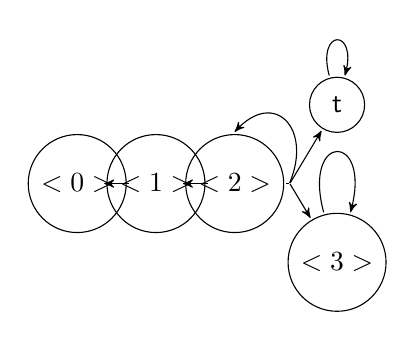
\begin{tikzpicture}[scale=1]
	
	\drawcirc (0) at (0,0) {$\state<0>$};
	\drawcirc (1) at (1,0) {$\state<1>$};
	\drawcirc (2) at (2,0) {$\state<2>$};
	\drawdummy (mid) at (2.7,0) {};
	\drawcirc (3) at (3.3,-1) {$\state<3>$};
	\drawcirc (t) at (3.3,1) {$\mathsf t$};
	
	\draw[->] (0) to (1);
	\draw[->] (1) to (2);
	\draw[-] (2) to (mid);
	
	\draw (mid) --  (t);% node [midway,anchor=north east] {0.5};
	\draw (mid) --  (3);%node [midway,anchor=south east] {0.5};
	\draw (mid) to [bend left,looseness=2,out=290,in=270] (2) ;
	
	\draw[->]  (3) to [loop above]  (3);
	\draw[->]  (t) to [loop above] (t) ;
	
	
	\end{tikzpicture}
} %\quad %
\subcaptionbox{\label{fig:VI_table}}
{	
	\begin{tabular}{c c c c}
		\toprule
		Iter. & $\lb(\state<0>)$ & $\lb(\state<1>)$ & $\lb(\state<2>)$\\ \midrule
		0	&	0			&	0			&	0			\\
		1	& 	0			& 	0			&	$\sfrac 1 3$	\\
		2	&	0			&	$\sfrac 1 3$	&	$\sfrac 4 9$ \\
		3	&	$\sfrac 1 3$	&	$\sfrac 4 9$ &	$\sfrac{13}{27}$\\
		4   &	$\sfrac 4 9$ & $\sfrac{13}{27}$ & $\sfrac{40}{81}$ \\ \bottomrule
	\end{tabular}
} %\quad %
\subcaptionbox{\label{fig:BVI_table}}
{	
	\begin{tabular}{c l l}
		\toprule
		Iter. & $\lb(\state<2>)$ & $\ub(\state<2>)$\\ \midrule
		0	&	0	 &	1		\\
		1	& 	0.01  & 0.99 			\\
		2	&	0.029~~& 0.980		\\
		3	&	0.039 & 0.970\\
		4   &	0.048 & 0.961	\\ \bottomrule
	\end{tabular}
}

\caption{(a) Example Markov chain (b) Under approximations computed by value iteration, see Example \ref{ex:vi} (c) Under- and over-approximations computed by bounded value iteration, see Example \ref{ex:bvi}.}
\end{figure}

\begin{example}\label{ex:vi}
	Consider the MC from Figure \ref{fig:VI_MC}, with $\trans(\state<2>,\state<2>)=\trans(\state<2>,\mathsf t)=\trans(\state<2>,\state<3>)=\frac 1 3$ and the reachability objective $\{t\}$.
	The estimates that VI computes in the first 4 iterations are depicted in Figure \ref{fig:VI_table}.
	The target state $\mathsf t$ is initialized to 1, everything else to 0. 
	The estimate for $\state<3>$ stays at 0, as it is a BSCC with no possibility to reach the target state.
	Since these two states do not change, they are omitted in the figure.
	In every iteration, the estimates are updated and become more precise, coming closer to the true value $0.5$ for $\state<0>$, $\state<1>$ and $\state<2>$.
	However, they converge to $0.5$ only in the limit, as for any finite number of iterations there is a positive probability to remain in $\state<2>$.
	Note that $\initstate$ always is two steps behind $\state<2>$, as it takes two iterations to backpropagate the current estimate.
	
\end{example}

VI converges to the true value only in the limit, hence we need some termination criterion $\TERMCRIT$ to stop when we are close enough. However, to be certain that the estimate is close, one has to perform an exponential number of iterations \cite{visurvey}, which is infeasible. Hence, usually this version of VI does not give convergence guarantees, but instead just runs until the difference between two successive iterations is small.
The result of this heuristic is guaranteed to be a lower bound, but can be arbitrarily imprecise~\cite{HM}, as we will also see in Example \ref{ex:bvi}.


\subsection{Bounded value iteration}
To be able to give convergence guarantees, \emph{Bounded value iteration} (BVI, also called interval iteration) was introduced more generally for Markov decision processes in \cite{atva14,HM}. In this paper, we only focus on Markov chains, i.e. Markov decision processes with a single action in every state. 
In addition to the under-approximation computed by VI, this approach also computes a convergent over-approximation. For this, it stores a second rational number for every state.
Dually to the under-approximation, $\INITIALIZE$ sets the estimate to 0 in states that cannot reach the target and 1 everywhere else. Note that finding the states with value 0, i.e. BSCC that do not contain the target, BVI has to perform a graph analysis, e.g. a backwards search from the targets.
BVI still works on the whole state space and the update is completely analogous to VI, only this time updating both approximations.
As $\TERMCRIT$, BVI checks that difference between the over- and under-approximation in the initial state is smaller than a given precision $\varepsilon$.
This guarantees that the returned value is $\varepsilon$-precise.

\begin{example}\label{ex:bvi}
		Consider the MC from Figure \ref{fig:VI_MC} with the same objective, but this time with 
		$\trans(\state<2>,\state<2>)= 0.98$ and $\trans(\state<2>,\mathsf t)=\trans(\state<2>,\state<3>) = 0.01$.
		Note that by pre-processing we set the over approximation $\ub(\state<3>)$ to 0, as it is a BSCC with no possibility of reaching the target. 
		The estimates BVI computes for $\state<2>$ in the first 4 iterations are depicted in Figure \ref{fig:BVI_table}.
		
		If we were running VI only from below, we might stop after iteration 4, as the lower bound changes by less than $0.01$ between these iterations and hence it seems to have converged close to the value.
		However, the difference between upper and lower bounds is still very high, so BVI knows that there still is a huge uncertainty in the values, as it could be anything between 0.048 and 0.961.
		Eventually, both estimates converge close enough to 0.5; for example, after around 400 iterations the lower bound is 0.49 and the upper bound 0.51. 
		Then BVI can return the value 0.5 (the center of the interval) with a precision of $0.01$, as this value is off by at most that.
\end{example}

\subsection{Simulation-based asynchronous value iteration}

The biggest drawback of the two variants we introduced so far is that they always work on the whole state space. 
Because of the state-space explosion, this is often infeasible.
In contrast, asynchronous value iteration only updates parts of the state space in every iteration of the loop, i.e. $\GETSTATES$ does not return the whole state space, but instead heuristically selects the states to update next.
This not only speeds up the main loop, but also allows the algorithm to reduce the memory requirements.
Indeed, instead of storing estimates for all states, one stores estimates only for the partial model consisting of previously updated states.
In~\cite{RTDP,BRTDP,atva14}, the heuristic for selecting the states is based on simulation: a path is sampled in the model, and only the states on that path are updated. 
The partial model contains all states that have been encountered during some of the simulations. 
If the part of the state space that is relevant for convergence of value iteration is small, this can lead to enormous speed-ups~\cite{atva14,cores}. For more details on why this happens and a formal definition of 'state space relevant for convergence', we refer the interested reader to~\cite{cores}.

\begin{algorithm}[htbp]
	\caption{Simulation-based implementation of $\GETSTATES$}\label{alg:simulate}
	\begin{algorithmic}[1]
		\Require{MC $\MC$, reachability objective $\targetset, \initstate$}
		\Ensure{A set of states $X \subseteq \states$}
		\Procedure{SIMULATE}{}
		\State $\path \gets \initstate$		
		\Repeat
		\State $\state' \gets$ sample from $\delta(\last{\path})$ according to $\nextstate$
		\State $\path \gets \path \state'$
		\Until{$\last{\path} \in \targetset$ or $\STUCK$}
		\State \Return $\path$
		\EndProcedure
	\end{algorithmic}
\end{algorithm}

Algorithm~\ref{alg:simulate} shows how states can be sampled through simulations, as done in \cite{atva14}:
Starting from the initial state, in every step of the simulation a successor is chosen from the distribution of the last state on the path. 
Note that this choice depends on another heuristic $\nextstate$. The successor can be chosen according to the transition probabilities $\delta$, but it has proven to be advantageous to additionally consider the difference between the upper and lower bound in the successor states \cite{BRTDP,atva14}. 
In consequence, states where we already know a lot (under- and over-approximations are close to each other) are given less priority than states where we still need information.

The simulation is stopped in two cases: Either (i) it reaches a target state or (ii) it is stuck in a BSCC with no path to the target.
Different heuristics for checking whether the simulation is stuck are discussed in depth in Section \ref{sec:stuck}.
Note that being able to differentiate between targets and non-target BSCCs during the simulations allows us not to do anything in $\INITIALIZE$; we can set the value to 1 when reaching a target and 0 in the other case.
The $\UPDATE$ function for simulation based asynchronous value iteration again uses the Bellman equation (\ref{eq:Vs}) to update the estimates of all states on the path; 
moreover, it can utilize additional information: Since $\GETSTATES$ returns a path, there is a notion of order of the states. Updating the states in reverse order backpropagates information faster.

\begin{figure}[t]
	\centering
\subcaptionbox{\label{fig:brtdp}}
{	
	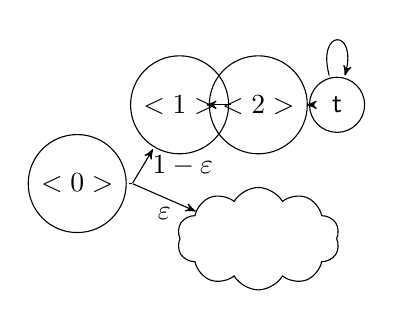
\begin{tikzpicture}[scale=1]
	
	\drawcirc (0) at (0,0) {$\state<0>$};
	\drawdummy (mid) at (0.7,0) {};
	\drawcirc (1) at (1.3,1) {$\state<1>$};
	\drawcirc (2) at (2.3,1) {$\state<2>$};
	\drawcirc (t) at (3.3,1) {$\mathsf t$};
	
	
	\node [cloud, draw,cloud puffs=10,cloud puff arc=120, aspect=2, inner ysep=1em] (cloud) at (2.3,-0.7) {};
	
	
	\draw[-] (0) to (mid);
	\draw[->] (mid) to node [midway,anchor=west] {$1 - \varepsilon$} (1);
	\draw[->] (mid) to node [midway,anchor=north] {$\varepsilon$} (cloud);
	\draw[->] (1) to (2);
	\draw[->] (2) to (t);

	\draw[->]  (t) to [loop above] (t) ;	
	
	\end{tikzpicture}
}\hspace{4em}
\subcaptionbox{\label{fig:adv}}
{	
	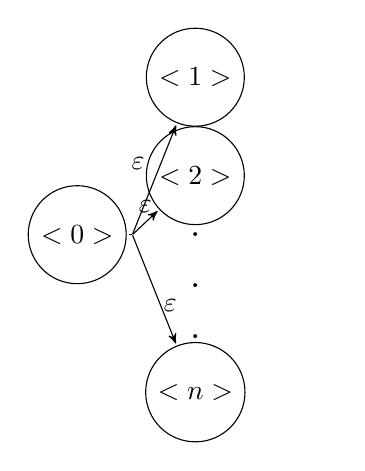
\begin{tikzpicture}[scale=1]
	
	\drawcirc (0) at (0,0) {$\state<0>$};
	\drawdummy (mid) at (0.7,0) {};
	\drawcirc (a) at (1.5,2) {$\state<1>$};
	\drawcirc (b) at (1.5,0.75) {$\state<2>$};
	\drawdummy (d1) at (1.5,0) {\Large .};
	\drawdummy (d2) at (1.5,-0.65) {\Large .};
	\drawdummy (d3) at (1.5,-1.3) {\Large .};
	%\drawcirc (c) at (1.5,-0.75) {$\mathsf t$};
	\drawcirc (d) at (1.5,-2) {$\state<n>$};
	\drawdummy (e) at (3.3,0) {};%to make pictures same width
	
	
	\draw[-] (0) to (mid);
	\draw[->] (mid) to node [midway,anchor=south east] {$\varepsilon$} (a);
	\draw[->] (mid) to node [midway,anchor=south ] {$\varepsilon$} (b);
	%\draw[->] (mid) to node [midway,anchor=north ] {$\varepsilon$} (c);
	\draw[->] (mid) to node [midway,anchor=north west ] {$\varepsilon$} (d);	
	
	\end{tikzpicture}
}
\caption{(a) A Markov chain where exploring the whole state space can be avoided. $\varepsilon$ denotes a transition probability. The cloud represents an arbitrarily large state space. (b) A Markov chain with high branching. From $\initstate$, there is a uniform probabilistic choice with $n = \frac {1} {\varepsilon}$ successors.}
\label{fig:brtdpAdv}
\end{figure}

\begin{example}
	Consider the MC in Figure \ref{fig:brtdp}, again with reachability objective $\{t\}$.
%	$\varepsilon$ and $1-\varepsilon$ denote transition probabilities.
	The cloud represents an arbitrarily large state space.
	However, since it is only reachable with a very small probability $\varepsilon$ (and we are interested in an $\varepsilon$-precise solution), it need not be explored.
	Let the first sampled path be $\state<0> \state<1> \state<2> \mathsf t$. This happens with high probability, as the only other possibility would be to select a successor from the cloud in state $\state<0>$, but since the selection process depends on the transition probabilities $\trans$, going to $\state<1>$ has a higher probability.
	After the simulation reaches $\mathsf t$, this value is backpropagated in reverse order. 
	First the lower estimate $\lb(\state<2>)$ is set to 1, then $\lb(\state<1>)$ is set to 1, then $\lb(\state<0>)$ is set to $1-\varepsilon$. 
	At this point the algorithm has converged, as difference between the lower and upper bound is~$\varepsilon$.
	
	So in this example, sampling the most probable path a single time gives a good approximation. The algorithm avoids exploring the large cloud and backprogagates values faster than synchronous VI.
\end{example}

\begin{example}\label{ex:adv}
	As an adversarial example, consider the MC in Figure \ref{fig:adv}.
	Here, the model exhibits high branching, so every single path has a low probability, and only by aggregating all paths we actually get a high value.
	Unlike the previous example, there is no part of the state space that is clearly irrelevant.
	In fact, to achieve precision of $\varepsilon$ the algorithm has to see so many paths that their cumulative probability is $1-\varepsilon$, which in this case means seeing all but one transition from the starting state. 
	This needs at least $\frac 1 \varepsilon$ simulations, but since the successors are chosen probabilistically, most likely a lot more.
\end{example}

Note that similarly to synchronous VI, there are versions of asynchronous VI without (RTDP \cite{RTDP}) and with  (BRTDP \cite{BRTDP,atva14})\footnote{While all are more generally applicable to Markov decision processes, \cite{BRTDP} only ensures convergence if no end components \cite{BK08} are present (for MC, no BSCCs without a target are present) and \cite{atva14} lifts this restriction.} guaranteed error bounds.
	
\subsection{Statistical model checking}

Algorithms for statistical model checking (SMC), \cite{Younes02}, are different from all previously described ones in two ways, namely what they store and what they return. 
The VI-based algorithms store estimates for every (seen) state and they update these values to be ever more precise.
Thus, the returned bounds on the values are certainly correct, although possibly quite loose.
In contrast, SMC stores only a single accumulator (for the value of the initial state) and the returned value is probably approximately correct (PAC \cite{pac}).
Being PAC with probability $\alpha$ and approximation $\epsilon>0$ guarantees the following:
with high probability ($\alpha$), the returned value is close to the true value (off by at most $\varepsilon$).
However, the returned confidence interval is not guaranteed to be a valid under- and over-approximation; 
if we are unlucky (i.e. with the remaining probability $1-\alpha$), there is no guarantee whatsoever on the returned value.

SMC does not need to do anything in $\INITIALIZE$.
It only stores a single accumulator to remember how often a target state was reached.
$\GETSTATES$ works as in Algorithm \ref{alg:simulate} with $\nextstate$ typically sampling the successor according to the transition probabilities $\trans$ (in some settings, importance sampling may also be possible, e.g. \cite{DBLP:conf/cav/JegourelLS12,DBLP:conf/setta/BuddeDH17}).
$\UPDATE$ remembers whether we reached the target or not; in the end we can divide the number of reaches by the total number of samples to get the probability estimate. 
$\TERMCRIT$ is a (typically low) number of samples that depends on the required probability of the guarantee and the width of the confidence interval; see \cite[Section 2.2]{DHKPjournal} for details or \cite{DBLP:journals/tomacs/JegourelSD19} for more advanced techniques.

\begin{example}\label{ex:smc}
	Consider again the MC depicted in Figure \ref{fig:VI_MC}.
    Let the first sampled path be $\state<0> \state<1> \state<2> \state<2> \mathsf t$. At this point the simulation stops, as we have reached a target state, and we remember that we have seen a target once.
    Let the second path be $\state<0> \state<1> \state<2> \state<2> \state<2> \state<3> \state<3> \dots$.
    On the one hand, the $\STUCK$ function has to let the simulation continue, even though $\state<2>$ is seen 3 times and it looks like a cycle.  
    On the other hand, it has to detect that the simulation will loop forever in $\state<3>$ and has to stop it.
    Ways to detect this are discussed in Section \ref{sec:stuck}.
    After detecting that we are stuck, we remember that the simulation did not reach the target.
        
    Let the required probability of the guarantee be $\alpha=0.9$ and the width of the confidence interval $\varepsilon=0.1$.
    Using Hoeffding's inequality \cite{hoeffding} we can show that the required number of samples for this is 461.
    So assume that after 461 simulations we have seen the target 223 times. 
    Then we know that with probability at least $0.9$, the value is in the interval $\sfrac {223} {461} \pm 0.05$, i.e. $[0.434,0.534]$.
    Increasing the number of simulations can both increase the confidence or decrease the width of the interval.
    
    Note that this number of simulations is independent of the system. While 461 simulations are a lot for this small system, the number would be the same if we were considering a model with several billion states where value iteration is impossible.
\end{example}



\section{STUCK}\label{sec:stuck}
In this section, we discuss heuristics for detecting whether a simulation is stuck in a BSCC with no path to a target state.
We also propose one new such heuristic with convenient theoretical properties.

For simulation-based asynchronous value iteration, previous work either excluded the existence of non-target BSCCs in their assumptions \cite{RTDP,BRTDP} or used a heuristic with no false negatives, but the possibility of false positives \cite{atva14}.
This means that if the simulation is stuck in a BSCC, the simulation definitely is stopped, which is required for termination. 
However, if the simulation is not stuck in a BSCC, it might still be stopped, guessing the value of the last state in the path is 0, although it might not be.
The $\STUCK$-heuristics used in previous work either depend on the path length (\cite{atva14}, \cite[Chapter 7.5]{ujma}) or simply stops exploring when any state is seen twice \cite[Appendix A.3]{cav19}.

SMC has to be sure with high probability that the simulation is stuck, as otherwise it loses the probabilistic guarantee.
In \cite{YCZ10}, two approaches are described. 
The first approach requires knowledge of the second eigenvalue of the MC in order to guarantee asymptotic convergence. However, getting the second eigenvalue is as hard as the verification problem itself.
The second approach works in the grey-box setting and pre-processes the MC so that all potentially infinite paths are eliminated.
A similar transformation, using white-box information, was suggested in \cite{ase10}.
However, both of these approaches transform the whole model and thus face problems in the case of very large models.
% The second approach of [26] requires the knowledge of the chain’s topology, which is used to transform the chain so that all potentially infinite paths are eliminated. In [9], a similar transformation is performed, again requir-ing knowledge of the topology. The (pre)processing of the state space required by the topology-aware methods, as well as by traditional numerical methods for Markov chain analysis, is a major practical hurdle for large (or unknown) statespaces

An alternative was suggested in \cite{DHKP16}.
It monitors the finite path sampled during the simulation, implicitly constructing a graph with all seen states as nodes and all seen transitions as edges.
The \emph{candidate} of the current path is the (possibly empty) set of states forming the maximal BSCC of this graph.
Intuitively, it is what we believe to be a BSCC given the observation of the current simulation. 
This candidate has to be validated, because as we saw in Example \ref{ex:smc}, a state set can look like a BSCC for several steps before being exited.
In the black-box setting, this validation works by continuing the simulation until the probability of overlooking some transition exiting the candidate becomes very small \cite{DHKP16}.

In this paper, we pinpoint that in the grey-box or white-box setting, this costly type of validation is not necessary. 
Instead of validating the candidate by running around in it for a huge number of steps, one can verify it using the additional information on the model. 
If no successor of any state in the candidate is outside of the candidate, then it indeed is a BSCC. 
Formally, for a candidate $T$, we check that $\{\state \mid \exists \mathsf t \in T: \state \in \post(t)  \} \subseteq T$ (if the topology is known), or alternatively that $\forall \mathsf t\in T: |\widehat{\post}(t)|=|\post(t)|$ (in what we defined as the grey-box setting) where $\widehat{\post}$ yields the number of successors within the observed candidate.

\begin{example}
	Consider again the MC depicted in Figure \ref{fig:VI_MC}.
	When a simulation enters $\state<3>$, $\STUCK$ should return true in order to stop the simulation, as it has reached a BSCC with no path to a target.
	In the black box setting of \cite{DHKP16}, this is only possible after continuing the simulation for another huge amount of steps. 
	For example, even in a BSCC with only a single state, hundreds of further steps can be necessary to reach the required confidence.
	Given the grey-box information, the algorithm can determine that all successors of the states in the candidate ($\{\state<3>\}$) have been seen and conclude that the candidate is indeed a BSCC.
\end{example}

However, this check stops the simulation and can incur an overhead if there are many SCCs in the transient part of the state space. 
Hence, we can delay it, not checking at the first occurrence of a cycle, but e.g. only when every state in the candidate has been seen twice.
Alternatively, one can only allow the check every $n$ (e.g. hundred) steps of the simulation.
Depending on the model and the implementation of the algorithm, these heuristics can have some impact on the runtime.
% we only want to perform it every $n$ steps or after getting a candidate of a certain \emph{strength} $k$, i.e. every state of the candidate was seen at least $k$ times.
%See Section~\ref{sec:discussion} for a discussion of the effect of these parameters. %\todo{this part kinda depends on what we want to say in discussion and what actually happens in experiments. Also check whether we actually keep the promise of investigating these parameters.}

Furthermore, one might modify this heuristic even further.
If a state of the BSCC is only reached with low probability, it takes many steps for the simulation to reach it.
When we check whether the current candidate is a BSCC, this state might not have occurred in the simulation yet. 
Instead of concluding that the information is insufficient and the simulation has to continue, one could deterministically explore the unknown successors and \emph{compute} the BSCC.
On the one hand, for small to medium sized BSCCs, this could result in a speed-up. 
%However, for large BSCCs or if the whole model forms an SCC, this could result in exploring the whole model.
On the other hand,  it increases the overhead when transient SCCs are checked by $\STUCK$.
%\todomaxi{I removed the comment on PRISM, cause we are not certain it is their fault. Also, the problem is not model construction, but checking whether some target is in the BSCC, as then you need to access model information, which takes a while. But we are not certain enough to say that, and it is not that interesting}
%, particularly costly in PRISM, where simulation and model construction do not work efficiently together.
Consequently, in the available benchmarks, this heuristic did not prove advantageous.
Hence we do not even report on it in the evaluation section.

%This STUCK also works for BRTDP. 
%\todo{Did we implement that? Do we have models were it makes a difference? Do we want to explicitly say this?}
	%Would have to have a large SCC in the transient part, which is hard to leave and always breaks the paths. 


\section{Discussion}\label{sec:discussion}


\subsection{Dependency of simulation length on topology}\label{sec:simBad}

Although the number of samples in SMC is independent of the model size, the length of the simulations is highly dependent on the model size and even more on the structure.
Indeed, any kind of cyclic behaviour in the transient part of the state space increases the simulation time for two reasons.
Firstly, the simulation loops in transient SCCs and does not make progress towards a target or a BSCC.
Secondly, the check whether the simulation is stuck in transient SCCs incurs an overhead.
An adversarial handcrafted worst-case example where simulations struggle is given in~\cite[Figure 3]{HM}.
Moreover, the structure of BSCCs affects the length of the simulation. 
For cyclic BSCCs, the simulation easily encounters all states of the BSCC and can quickly terminate.
For more complex topologies, some states are typically only seen with very low frequency and thus the simulation takes longer.

If the model exhibits many transient SCCs, using any simulation-based technique is problematic. 

\subsection{Black, grey and white SMC}

The difference between the variants of SMC we report on are their knowledge of the transition system: $\pmin$ corresponds to black, the number of successors to grey and the exact successors and probabilities to the white-box setting.
This information can be used in the $\STUCK$-check; apart from that, the algorithms are the same.

%Our heuristic using the additional information of the white box setting did not speed up the algorithm, as the overhead for the additional checks was too large, see end of Section \ref{sec:stuck}.


Comparing grey and black box, it is apparent that simulations in grey box can be much shorter, as upon detection of a candidate that is a BSCCs the simulation is immediately stopped, whereas in the black box setting it has to continue for a number of steps.
This number of steps depends on two things: (i) The size of the BSCC, as larger BSCC take longer to explore, especially since all states, no matter how improbable, need to be seen a certain amount of times, and (ii) the given under-approximation of the minimum transition probability $p_{min}$, as this determines how often every state in the candidate has to be seen until the probability of a false positive is small enough.

Thus, for large BSCCs or small $\pmin$, grey SMC is clearly better, as we also experimentally validate in Table \ref{tab:herman-short} (large BSCC) and Table \ref{tab:fsmc-vary-pmin} (various $\pmin$) in the next section.
For small BSCCs (e.g. only of size 1) and not so small $p_{\min}$, black and grey SMC become more comparable, but grey SMC still has shorter simulations.
However, practically, the overhead of verifying the candidates in grey SMC can be so large that black SMC can even be slightly faster than grey SMC (see e.g., \texttt{leader6\_11} in Table \ref{tab:grey-v-black}).

Heuristically reducing the number of checks in grey SMC (as described in Section \ref{sec:stuck}) can make it faster again, but the effectiveness of the heuristics depends on the models. 
So, if it is known that the BSCC-detection is very easy for black SMC (e.g. they are of size 1 or cyclic and $\pmin$ is not too small), black SMC can be a viable choice. 
However, as black SMC is never far better, using grey SMC is the safer variant when facing models with uncertain topology.

\subsection{Comparison of algorithms}
%\todo{DT/Table for algo selection in final version?}
Finally, we compare the (dis-)advantages of the different algorithms, giving a practical decision guidance.
If hard guarantees are required, then  BVI or BRTDP are to be used.
The latter is simulation based, and thus good if only a small part of the state space is relevant for convergence. 
Additionally, if the model is too large for BVI, BRTDP still has a chance, but quite possibly the partial model will also be too large.
Conversely, if the model contains lots of transient SCCs, BVI is preferable, as simulation based approaches fail on this kind of model, see Section \ref{sec:simBad}.
Note that, if there are small probabilities present, it might take very long for BVI and BRTDP to converge, see Example \ref{ex:bvi}.

For a quick estimate, or if PAC guarantees are sufficient, or if the system is too large, so that it is not possible to provide hard guarantees, SMC is to be used, if possible (white or grey box setting) in our grey variant.
As both the memory and the termination criterion are independent of the size of the system, SMC always has a chance to yield an estimate, which additionally comes with a probabilistic guarantee.

There is no case in which un-guaranteed (synchronous or asynchronous) VI are preferable, as they suffer from the same drawbacks as BVI and BRTDP, but additionally do not provide guarantees.
Whenever hard guarantees are not of interest and the system is not strongly connected, grey SMC should be used for a quick estimate.
%Whenever guarantees are not of interest, SMC yields the quickest estimate. => Actually not true, see exp; hermann17 has 130,000 states, but VI is faster.


\subsection{Extensions to other unbounded-horizon properties}
	For more complex unbounded-horizon properties \cite{BK08}, such as Until (avoid-reach), LTL or long-run average reward, (B)VI pre-processes the state space to analyze the BSCCs \cite{BK08} and BRTDP \cite{atva14} can either do the same  or analyze the encountered BSCCs only. 
	Black SMC of \cite{DHKPjournal} is applicable through additional analysis of the BSCC candidates after they have been found likely to be BSCCs.
	This is directly inherited by grey SMC and makes it available for these specifications with low overhead.



%\para{INITIALIZE:}
%For VI, set the initial values. 
%For BRTDP and our SMC, nothing.
%For the other SMC, precompute 0 states.
%
%
%\para{TERM\_CRIT:}
%For VI and BRTDP, $\varepsilon$-convergence.
%For SMC, necessary number of samples.
%
%\para{GET\_STATES:}
%For VI: Everything.
%For BRTDP and SMC: Sample path until target or STUCK.
%
%\para{STUCK:}
%For BRTDP: Some heuristic (increasing path length, state seen twice...)
%For SMC: Depends. Can be our white thing (with different ideas), can be the candidate thing, can be importance sampling or whatever else there exists.
%Different ideas: When we think we have candidate: Check. If true, done. Else: Continue simulation/Unfold for n steps.
%
%\para{UPDATE}
%For VI: Bellman backup
%For BRTDP: Infer value of place where path ended. (Might use STUCK ideas), then Bellman backup.
%For SMC: Remember whether target or STUCK.





\section{Experimental evaluation}\label{sec:experiments}

%Exp:
%prob0 then VI
%prob0 then SMC
%BRTDP
%Black SMC
%White SMC

%Models:
%QComp? Large MC with lots of branching
%PRISM bench suite (Check there is nothing?)
%handcraft sth
%Pepa?
%Hermann self-stabilization

We implemented grey SMC in a branch of the PRISM Model Checker \cite{prism} extending the implementation of black SMC \cite{DHKPjournal}.
We ran experiments on (both discrete- and continuous-time) Markov chains from the PRISM Benchmark Suite \cite{prism-benchmark-suite}.
In addition to a comparison to black SMC, we also provide comparisons to VI and BVI of PRISM and BRTDP of \cite{atva14}.
An interested reader may also want to refer \cite[Table II]{DHKPjournal} for a comparison of black SMC against two unbounded SMC techniques of \cite{YCZ10}.

For every run configuration, we run 5 experiments and report the median.
In black SMC, the check for candidates is performed every 1000 steps during path simulations, while in grey SMC the check is performed every 100 steps.
Additionally, grey SMC checks if a candidate is indeed a BSCC once every state of the candidate is seen at least twice.
In all our tables, `TO' denotes a timeout  of 15 minutes and `OOM' indicates that the tool ran out of memory restricted to 1GB RAM.

\subsection{Comparison of black and grey SMC}

% Please add the following required packages to your document preamble:
% \usepackage{booktabs}
% \usepackage{lscape}
\begin{table}[t]
\centering
\caption{Runtime (in seconds) comparison of black and grey SMC for various benchmarks. BVI runtimes are also presented as a baseline.}
\label{tab:grey-v-black}
\setlength{\tabcolsep}{6pt} % Default value: 6pt
\begin{tabular}{@{}l@{\hspace{-0.5em}}rrrrrr}
	\toprule
	Model/                                  &    Size &               $\pmin$ &             BSCC & \multicolumn{2}{c}{SMC} & BVI \\
	\cmidrule(lr){5-6}
	Property                                &         &                       & (No., Max. Size) & Black &            Grey &     \\ \midrule
	\texttt{bluetooth(10)}                  & $>569K$ & $7.81 \times 10^{-3}$ &       $>5.8K, 1$ &     9 &               \textbf{7} &  TO \\
	\vspace{0.5em}
	\texttt{time\_qual}                     &         &                       &                  &       &                 &     \\
	\texttt{brp\_nodl(10K,10K)}             &  $>40M$ &    $1 \times 10^{-2}$ &       $>4.5K, 1$ &    86 &              \textbf{84} &  TO \\
	\vspace{0.5em}
	\texttt{p1\_qual}                       &         &                       &                  &       &                 &     \\
	\texttt{crowds\_nodl(8,20)}             &     68M &    $5 \times 10^{-2}$ &         $>3K, 1$ &    10 &               \textbf{8} &  TO \\
	\vspace{0.5em}
	\texttt{positive\_qual}                 &         &                       &                  &       &                 &     \\
	\texttt{egl(20,20)}                     &   1719T &    $5 \times 10^{-1}$ &           $1, 1$ &    43 &              \textbf{25} &  TO \\
	\vspace{0.5em}
	\texttt{unfairA\_qual}                  &         &                       &                  &       &                 &     \\
	\texttt{gridworld(400,0.999)}           &    384M &    $1 \times 10^{-3}$ &      $796, 160K$ &    15 &               \textbf{8} &  TO \\
	\vspace{0.5em}
	\texttt{prop\_qual}                     &         &                       &                  &       &                 &     \\
	\texttt{herman-17}                      &     10G &  $4.7 \times 10^{-7}$ &          $1, 34$ &    TO &              \textbf{73} &  98 \\
	\vspace{0.5em}
	\texttt{4tokens}                        &         &                       &                  &       &                 &     \\
	\texttt{leader6\_11}                    & $>280K$ &  $5.6 \times 10^{-7}$ &           $1, 1$ &   \textbf{106} &             152 & OOM \\
	\vspace{0.5em}
	\texttt{elected\_qual}                  &         &                       &                  &       &                 &     \\
	\texttt{nand(50,3)}                     &     11M &    $2 \times 10^{-2}$ &          $51, 1$ &    11 &              \textbf{10} & 455 \\
	\vspace{0.5em}
	\texttt{reliable\_qual}                 &         &                       &                  &       &                 &     \\
	\texttt{tandem(2K)}                     & $>1.7M$ &  $2.4 \times 10^{-5}$ &       $1, >501K$ &     \textbf{7} &               \textbf{7} &  62 \\
	\texttt{reach\_qual}                    &         &                       &                  &       &                 &     \\ \bottomrule
\end{tabular}
\end{table}
 
% Please add the following required packages to your document preamble:
% \usepackage{lscape}
\begin{table}[t]
	\centering
	\caption{Effect of $\pmin$ on black SMC runtimes (in seconds) on some of the benchmarks. Lower $\pmin$ demands stronger candidates, due to which black SMC has to sample longer paths.}
	\label{tab:fsmc-vary-pmin}
	\setlength{\tabcolsep}{10pt} % Default value: 6pt
	\begin{tabular}{@{}lrrrrr@{}}
		\toprule
		                                           &                             \multicolumn{4}{c}{Black SMC/$\pmin$}  & \multirow{2}{*}{Grey SMC}                           \\
		\cmidrule(l){2-5}
		Model & $1 \times 10^{-2}$ & $1 \times 10^{-3}$ & $1 \times 10^{-4}$ & $1 \times 10^{-5}$ &  \\ \midrule
		\texttt{brp\_nodl(10K,10K)}         & 86                & 93                 & 183                & TO    & \textbf{84}             \\
		\texttt{crowds\_nodl(8,20)}         & 11                 & 41                 & 334                & TO     & \textbf{9}            \\
		\texttt{egl(20,20)}                 & 47                 & 106                 & 875                & TO     & \textbf{44}            \\ \bottomrule
	\end{tabular}
\end{table}


Table \ref{tab:grey-v-black} compares black SMC and grey SMC on multiple benchmarks. 
One can see that, except in the case of \texttt{leader6\_11} and \texttt{brp\_nodl}, grey SMC finishes atleast as soon as black SMC.
In \texttt{bluetooth}, \texttt{gridworld}, \texttt{leader} and \texttt{tandem}, both the SMC methods are able to terminate without encountering any candidate (i.e. either the target is seen or the left side of the until formula is falsified).
In \texttt{brp\_nodl}, \texttt{crowds\_nodl} and \texttt{nand}, the SMC methods encounter a candidate, however, since the candidate has only a single state (all BSCCs are trivial), black SMC is quickly able to confidently conclude that the candidate is indeed a BSCC.
The only interesting behaviour is observed on the \texttt{herman-17} benchmark. 
In this case, every path eventually encounters the only BSCC existing in the model.
Grey SMC is able to quickly conclude that the candidate is indeed a BSCC, while black SMC has to sample for a long time in order to be sufficiently confident.

The performance of black SMC is also a consequence of the $\pmin$ being quite small. 
Table \ref{tab:fsmc-vary-pmin} shows that black SMC is very sensitive towards $\pmin$.
Note that grey SMC is not affected by the changes in $\pmin$ as it always checks whether a candidate is a BSCC as soon as all the states in the candidate are seen twice.


%Better if large BSCC or small pmin.
%But also Black SMC often good.

%various checkBound (how often to check): 1, 10, 100, 1000
%various simminvisits (strength of candidate): 0, 2, 5, 20, 100, 1000

%always report [min/mean/max]

\subsection{Grey SMC vs. Black SMC/BRTDP/BVI/VI}

% Please add the following required packages to your document preamble:
% \usepackage{booktabs}
% \usepackage{lscape}
\begin{table}[t]
\centering
\caption{Runtime (in seconds) of the various algorithms on the Herman self-stabilization protocol \cite{HermanPrism} with the property \texttt{4tokens}. The median runtimes are reported for grey SMC, black SMC \cite{DHKPjournal}, BRTDP \cite{atva14}, Bounded value iteration (BVI) and Value iteration (VI). The SMC algorithms use SPRT method with parameters $\alpha = 0.01$ and $\beta = 0.01$. BRTDP, BVI and VI run until  a relative error of 0.01 is obtained.}
\label{tab:herman-short}
\setlength{\tabcolsep}{6pt} % Default value: 6pt
\setlength{\aboverulesep}{0pt}
\setlength{\belowrulesep}{0pt}
\begin{tabular}{@{}lrrr|rrr@{}}
	\toprule
	Model     & States & Grey SMC & Black SMC & BRTDP & BVI &  VI \\ \midrule
	\texttt{herman-5}     & 32 &       11 &   15 &    TO &   1 &   1 \\
	\texttt{herman-7}     & 128 &       12 &   57 &    TO &   1 &   1 \\
	\texttt{herman-9}     & 512 &       10 &  775 &    TO &   1 &   1 \\
	\texttt{herman-11}     & 2048 &       19 &   TO &    TO &   1 &   1 \\
	\texttt{herman-13}     & 8192 &       18 &   TO &    TO &   1 &   1 \\
	\texttt{herman-15}     & 33K &       17 &   TO &    TO &   9 &   3 \\
	\texttt{herman-17}     & 131K &       49 &   TO &    TO &  98 &  21 \\
	\texttt{herman-19}     & 524K &      252 &  OOM &    TO &  602 & 113 \\
	\texttt{herman-21}     & 2M &      759 &  OOM &   OOM &  TO &  TO \\ \bottomrule& 
\end{tabular}
\end{table}


We now look more closely at the self-stabilization protocol \texttt{herman} \cite{HermanPrism,Herman90}. 
The protocol works as follows:
\texttt{herman-N} contains N processes, each possessing a local boolean variable $x_i$. 
A token is assumed to be in place $i$ if $x_i = x_{i-1}$.
The protocol proceeds in rounds.
In each round, if the current values of $x_i$ and $x_{i-1}$ are equal, the next value of $x_i$ is set uniformly at random, and otherwise it is set equal to the current value of $x_{i-1}$.
The number of states in \texttt{herman-N} is therefore $2^N$.
The goal of the protocol is to reach a stable state where there is exactly one token in place. 
For example, in case of \texttt{herman-5}, a stable state might be $(x_1=0, x_2=0, x_3=1, x_4=0, x_5=1)$, which indicates that there is a token in place 2. 
In every \texttt{herman} model, all stable states belong to the single BSCC. 
The number of states in the BSCC range from 10 states in \texttt{herman-5} to 2,000,000 states in \texttt{herman-21}.

For all \texttt{herman} models in Table \ref{tab:herman-short}, we are interested in checking if the probability of reaching an unstable state where there is a token in places 2-5, i.e. $(x_1=1, x_2=1, x_3=1, x_4=1, x_5=1)$ is less than 0.05.
This property, which we name \texttt{4tokens}, identifies $2^{N-5}$ states as target in \texttt{herman-N}.
The results in Table \ref{tab:herman-short} show how well grey SMC scales when compared to black SMC, BRTDP, BVI\footnote{We refrain from comparison to other guaranteed VI techniques such as sound VI \cite{DBLP:conf/cav/QuatmannK18} or optimistic VI \cite{DBLP:journals/corr/abs-1910-01100} as the implementations are not PRISM-based and hence would not be too informative in the comparison.} and VI.
Black SMC times out for all models where $N \geq 11$. This is due to the fact that the larger models have a smaller $\pmin$, thereby requiring black SMC to sample extremely long paths in order to confidently identify candidates as BSCCs.
BVI and VI perform well on small models, but as the model sizes grow and transition probabilities become smaller, propagating values becomes extremely slow.
Interestingly, we found that in both grey SMC and black SMC, approximately 95\% of the time is spent in computing the next transitions, which grow exponentially in number; an improvement in the simulator implementation can possibly slow down the blow up in run time, allowing for a fairer comparison with the extremely performant symbolic value iteration algorithms.

\begin{table}[t]
\centering
\caption{Effect of restrictive properties (satisfied in fewer states) on the runtime (in seconds) of BRTDP in the herman benchmarks.}
\label{tab:herman-brtdp}
\setlength{\tabcolsep}{10pt} % Default value: 6pt
\begin{tabular}{@{}lrrr@{}}
	\toprule
	& \multicolumn{3}{c}{Property}\\
	\cmidrule(l){2-4}
Model                & \texttt{2tokens} & \texttt{3tokens} & \texttt{4tokens} \\
\midrule
\texttt{herman-5} & 1                  & 2                     & TO                   \\
\texttt{herman-7} & 1                  & 1                     & TO                   \\
\texttt{herman-9} & 1                  & 2                     & TO                   \\
\texttt{herman-11} & 2                  & 2                     & TO                   \\
\texttt{herman-13} & 2                  & 2                     & TO                   \\
\texttt{herman-15} & 3                  & 3                     & TO                   \\
\texttt{herman-17} & 5                  & 6                     & TO                   \\
\texttt{herman-19} & 9                   & 9                     & TO                   \\
\texttt{herman-21} & 104                 & 111                   & TO                   \\
\texttt{herman-23} & OOM                   & OOM                   & OOM                  
\\ \bottomrule
\end{tabular}
\end{table}

Finally, we comment on the exceptionally poor performance of BRTDP on \texttt{herman} models. 
In Table \ref{tab:herman-brtdp}, we run BRTDP on three different properties: (i) tokens in places 2-3 (\texttt{2tokens}); (ii) tokens in places 2-4 (\texttt{3tokens}); and (iii) tokens in places 2-5 (\texttt{4tokens}). 
The number of states satisfying the property decrease when going from 2 tokens to 4 tokens.
The table shows that BRTDP is generally better in situations where the target set is larger. %\todojan{quick jump to the conclusion; must be refined (or dropped)}

In summary, the experiments reveal the following:
\begin{itemize}
	\item For most benchmarks, black SMC and grey SMC perform similar, as seen in Table \ref{tab:grey-v-black}. 
	As expected, the advantages of grey SMC do not show up in these examples, which (almost all) contain only trivial BSCCs.
	\item The advantage of grey SMC is clearly visible on the \texttt{herman-N} benchmarks, in which there are non-trivial BSCCs. Here, black SMC quickly fails while grey SMC is extremely competitive.
	\item Classical techniques such as VI and BVI fail when either the model is too large or the transition probabilities are too small.
	However, they are still to be used for strongly connected systems, where the whole state space needs to be analysed for every run in both SMC approaches, but only once for (B)VI.%\todojan{I want to add this, although maybe we don't have data here; Maxi: I see the point, but not sure that "only once" is correct. It still takes several iterations, and every iteration works on the whole state space.}
\end{itemize}

\section{Conclusion}

While SMC has found its use also in the white-box setting as a scalable alternative, we introduce the first approach that utilizes the knowledge in a local way, without globally processing the state space, and thus preserves the efficency advantages of black-box SMC.
We call this approach grey SMC since we utilize only the topological information and not the quantitative information (sometimes referred to as grey box).
On the one hand, this is useful as the quantitative information is often unavailable or imprecise w.r.t.\ the modelled reality.
On the other hand, while the full quantitative information is irrelevant in BSCCs, it plays a major role in the transient phase and could be used to further enhance the approach. For instance, it could be used for importance sampling in order to handle rare events efficiently \cite{DBLP:conf/cav/JegourelLS12,DBLP:conf/setta/BuddeDH17} even in the context of unbounded-horizon properties.



\bibliographystyle{alpha}
%\bibliographystyle{splncs04}
\bibliography{ref,survey}

%\pagebreak
%\appendix
%\section*{Appendix}
%\input{appendix.tex}

\end{document}
